\documentclass[letterpaper]{book}

\usepackage[dvips]{graphicx}
\usepackage{epsfig} % for epsfig
\usepackage{amsmath}
\usepackage{amssymb}
\usepackage{graphicx}
\usepackage[usenames]{color}
%\graphicspath{{figures/}}

\newcommand{\dt}{\ensuremath{\delta t}}
\newcommand{\ddt}[1]{\frac{\partial #1}{\partial t}}
\newcommand{\thimp}{\ensuremath{\theta}}

\newcommand{\order}[1]{\ensuremath{\mathcal{O}(#1)}}

\renewcommand{\vec}[1]{\ensuremath{\mathbf{#1}}}
\newcommand{\tensor}[1]{\mathsf{#1}}
\newcommand{\tor}{\varphi}              % toroidal coordinate
\newcommand{\A}{\vec{A}}
\newcommand{\B}{\vec{B}}
\newcommand{\E}{\vec{E}}
\newcommand{\R}{\vec{R}}
\newcommand{\x}{\vec{x}}
\renewcommand{\r}{R}
\renewcommand{\v}{\vec{v}}
\renewcommand{\u}{\vec{u}}
\newcommand{\F}{\vec{F}}
\renewcommand{\j}{\vec{J}}
\newcommand{\q}{\vec{q}}
\newcommand{\g}{\vec{g}}
\newcommand{\jn}{\frac{\j}{n}}
\renewcommand{\P}{\tensor{\Pi}}
\renewcommand{\b}{\vec{b}}
\newcommand{\W}{\tensor{W}}
\newcommand{\codename}{\textsc{M3D-$C^1$}}

\newcommand{\grad}[1]{\nabla #1}
\newcommand{\gradp}[1]{\nabla_\perp #1}
\renewcommand{\div}[1]{\nabla \cdot #1}
\newcommand{\divp}[1]{\nabla_\perp \cdot #1}
\newcommand{\curl}[1]{\nabla \times #1}

\newcommand{\dotdot}{:}
\newcommand{\dottimes}{\dot\times}
\newcommand{\timestimes}{\stackrel{\times}{\times}}

\newcommand{\gs}[1]{\Delta^* #1}
\newcommand{\lp}[1]{\nabla^2 #1}
\newcommand{\pb}[2]{\left[#1,#2\right]}
\newcommand{\ip}[2]{\left\langle  #1,#2\right\rangle}
\newcommand{\funcss}[2]{
  \left\langle\left\langle #1,#2 \right\rangle\right\rangle}
\newcommand{\funcsa}[2]{\left[\left\langle #1,#2 \right\rangle\right]}
\newcommand{\funcaa}[2]{\left[\left[ #1,#2 \right]\right]}

\newcommand{\cola}[1]{\textcolor{Red}{#1}}
\newcommand{\colb}[1]{\textcolor{Blue}{#1}}

\newcommand{\uvec}[1]{\ensuremath{\vec{\hat{#1}}}}
\newcommand{\n}{\ensuremath{\uvec{n}}}


\newcommand{\repositoryloc}{portal.pppl.gov/p/tsc/C1/svn}
\newcommand{\svnurl}{http://subversion.tigris.org/}


\title{\codename\ User's Guide}
\author{Nathaniel M. Ferraro}

\begin{document}

\maketitle

\setcounter{tocdepth}{1}
\tableofcontents

\section{Download and Compilation}

%%%%%%%%%%%%%%%%%%%%%%%%%%%%%%%
\subsection{Accessing PPPL Machines}
%%%%%%%%%%%%%%%%%%%%%%%%%%%%%%%

Once you obtain a PPPL Unix user account, please visit the website:   
\newline\newline
\href{http://researchcomputing.pppl.gov}{http://researchcomputing.pppl.gov}
\newline\newline
There, you will find instructions for installing NX virtual Desktop.
\newline\newline
In PPPL machine, first get an interactive session for a single processor on the \texttt{portal} computer.    
The M3DC1 code is located in the Github repository: \texttt{PrincetonUniversity/M3DC1}. 
Access to this repository requires a Github account and permission from \href{mailto:nferraro@pppl.gov}{Dr. Nate Ferraro}. 
Note that Section \ref{ch:preinstall} describes how to use pre-compiled versions of M3D-C$^{1}$ so you do not need githup access.

%%%%%%%%%%%%%%%%%%%%%%%%%%%%%%%
\subsection{Github}
%%%%%%%%%%%%%%%%%%%%%%%%%%%%%%%

Retrieve the current version of M3D-C$^{1}$ from the GIT repository.  For the first time, to check out the sources do:
\begin{description}
\item[ ] Initial access is with the \texttt{clone} command.   This copies the source code from the master file into a working directory on your machine.   You only do this once on each computer you work on.
\item[ ] \texttt{module load git}
\item[ ] \texttt{git clone https://github.com/PrincetonUniversity/M3DC1}
\end{description}

Subsequent GIT commands used to commit:
\begin{description}
\item[ ] \texttt{add/commit/push}
you \texttt{add} files to a list of files to update, \texttt{commit} the changes to your branch, and then \texttt{push} the changes to the master branch
\item[ ] \texttt{git commit -m ``message describing changes''} (adding -a commits all changes)
\item[ ] \texttt{diff} lists the changes you made from the last commit, even if you haven't pushed your commits to github.    
   To see how your files differ from what's on github, you can do:
\begin{description}
\item[ ] \texttt{git fetch origin master}
\item[ ] \texttt{git diff origin/master}
\end{description}
\item[ ] \texttt{status} compares your branch with the master branch
\item[ ] \texttt{pull} updates your local branch to the current master branch
\newline
\texttt{	may need to origin master}
\item[ ] \texttt{stash} takes uncommitted changes, saves them for later use, and reverts files in working directory
\newline
\texttt{stash list	stash drop	stash apply	stash pop (apply+drop)}
\item[ ] \texttt{stash pop} removes changes from your stash and reapplies them to working copy
\item[ ] \texttt{stash apply} keeps changes in stash, but reapplies them to working copy
\item[ ] \texttt{reset -hard} discards any changes to local branch since last commit
\item[ ] \texttt{branch} tells you what branch you are in
\item[ ] \texttt{log} (--oneline) (--after 2017-12-31) lists all the commits for the checked-out branch after that date
\newline
log -pretty=format: ``\%h - \%an, \%ar : \%s''
\item[ ] \texttt{checkout} b8d17c0 switches to commit branch b8d17c0
\end{description}

%%%%%%%%%%%%%%%%%%%%%%%%%%%%%%%
\subsubsection{Branches in git}
%%%%%%%%%%%%%%%%%%%%%%%%%%%%%%%

To make a new branch called fp\_phase2
\\==========================================
\\\texttt{> git checkout master} \# switch to the master branch
\\\texttt{> git pull}  \# make sure the master branch is up-to-date
\\\texttt{> git checkout -b fp\_phase2} \# The ``-b'' create a new branch
\\\#   this will be identical to master to start
\\\texttt{> git push --set-upstream origin fp\_phase2} 
\\\# push this new branch to the remote repo so others can access it
\newline\newline
Committing changes (e.g., newpar.f90)
\\===========================================
\\
\texttt{> git pull}                           \# Always do this before you start committing
\\\#   if you forget, you risk diverging your local branch from remote
\\
\texttt{> git add newpar.f90} \# This stages the current changes in newpar.f90 for commit
\\\#   you could then make more changes before committing,
\\\#   but you'd have to add again to get those into the commit
\\
\texttt{> git commit -m "Changed newpar.f90"} \# Commit changes to your local branch 
\\
\texttt{> git push}                           \# Push commits to the remote repo
\\\#   ---set-upstream only needs to be done the first time
\newline\newline
Merge changes on master into fp\_phase2 (e.g., some important bug fix)
\\===========================================
\\\texttt{> git checkout master}    \# switch to the master branch
\\\texttt{> git pull}               \# get the latest commits on the master branch
\\\texttt{> git checkout fp\_phase2} \# switch back to fp\_phase2 (no need for -b now)
\\\texttt{> git pull}               \# get latest commits on fp\_phase2 to avoid conflicts
\\\texttt{> git merge master}       \# merge any new commits into fp\_phase2
\\\#  - this makes a commit
\\\#  - you may need to resolve conflicts
\\\texttt{> git push}               \# push the merge commit to remote repo
\newline\newline
Inverting fp\_phase2 and master here would merge the development branch into master locally, then the push would send the merge to the remote master.

%%%%%%%%%%%%%%%%%%%%%%%%%%%%%%%
\subsection{On-line Documentation}
%%%%%%%%%%%%%%%%%%%%%%%%%%%%%%%
An extensive document that describes equations solved by the code and the input variables in \texttt{"C1input"} is in the GIT repo. Please refer to: \texttt{\ldots/trunk/unstructured/doc/doc.pdf}
\newline\newline
Machine-specific instructions for portal, perseus, Edison, Cori are in:  
\texttt{\ldots/trunk/unstructured/README}
\newline\newline
Additional documentation is available on the site: \href{http://w3.pppl.gov/~nferraro}{http://w3.pppl.gov/$\sim$nferraro} under the ``M3D-C$^{1}$'' tab.
\newline\newline
The latest copy of his document is available at: \href{http://m3dc1.pppl.gov}{http://m3dc1.pppl.gov}

%%%%%%%%%%%%%%%%%%%%%%%%%%%%%%%
\subsection{Compilation}
%%%%%%%%%%%%%%%%%%%%%%%%%%%%%%%

%%%%%%%%%%%%%%%%%%%%%%%%%%%%%%%
\subsubsection{Load Modules}
%%%%%%%%%%%%%%%%%%%%%%%%%%%%%%%
\begin{itemize}
\item{\texttt{PPPL RHEL6 machines (portal.pppl.gov)}}
\newline\newline
\texttt{[openmpi-1.8.4]}
\\Load the following modules and copy sunfire.openmpi-1.8.4.mk to sunfire.pppl.gov.mk
\newline\newline
\texttt{
openmpi/1.8.4 intel/2015.u1 gsl/1.16 szip/2.1 hdf5-parallel hdf/4.2r1 
\\
scalapack	fftw			
}
\newline\newline
See README/readme.portalr.openmp-1.8.4 for detailed instructions and an example job script
\newline\newline
\texttt{[openmpi-1.10.3]}
\\
Load the following modules and copy sunfire.openmpi-1.10.3.mk to sunfire.pppl.gov.mk
\newline\newline
\texttt{openmpi/1.10.3 intel/2015.u1 gsl szip hdf5-parallel/1.8.17 
}
\newline\newline
See README/readme.portal.openmp-1.10.3 for detailed instructions and an example job script.
\newline\newline
\texttt{[openmpi-4.0.1]}
\\
Load the following modules and copy sunfire.openmpi-1.10.3.mk to sunfire.pppl.gov.mk
\newline\newline
\texttt{
openmpi/4.0.1 intel/2019.u3 gsl	szip scalapack 
}
\newline\newline
See README/readme.portal.openmp-4.0.1 for detailed instructions and an example job script.
%%%%%%%%%%%%%%%%%%%%%%%%%%%%%%%
\item{\texttt{PPPL RHEL7 machines (portalc7.pppl.gov)}}
%%%%%%%%%%%%%%%%%%%%%%%%%%%%%%%
\newline\newline
Load the following modules and copy \texttt{centos7.mk} to \texttt{sunfire.pppl.gov.mk}
\newline\newline
\texttt{openmpi/4.0.3 intel/2019.u3 hdf5-parallel/1.10.5 
}
\newline\newline
See README/readme.centos7 for detailed instructions and an example job script.

\item{\texttt{cori.nersc.gov}}
\newline\newline
See \texttt{README/readme.cori} and \texttt{README/readme.corigpu} for detailed instructions and an example job script.

\item{\texttt{perseus.princeton.edu}}
\newline\newline
Follow the instructions in \ref{ch:setup-idl} in first setting up idl 
\\
Load the following modules:
\newline\newline
\texttt{intel/18.0/64/18.0.3.222 intel-mpi/intel/2018.3/64 gsl/2.4
\\
hdf5/intel-17.0/intel-mpi/1.10.0	fftw/intel-16.0/intel-mpi/3.3.4
}
\newline\newline
See README/readme.perseus for detailed instructions and an example job script.
\\
For help regarding perseus, send email to: \href{mailto:cses@princeton.edu}{cses@princeton.edu}
\item{\texttt{perseus-amd.princeton.edu}}
\newline\newline
Load the following modules:
\newline\newline
\texttt{
intel/18.0/64/18.0.3.222 intel-mpi/intel/2018.3/64 gsl
\\
hdf5/intel-17.0/intel-mpi/1.10.0	fftw/intel-16.0/intel-mpi/3.3.4
}\\
See README/readme.perseusamd for detailed instructions and an example job script.
\newline\newline
For help regarding perseus, send email to: \href{mailto:cses@princeton.edu}{cses@princeton.edu}

\item{\texttt{stellar.princeton.edu}}
\newline\newline
See README/readme.stellar for detailed instructions and an example job script.
\\
For help regarding stellar, send email to: \href{mailto:cses@princeton.edu}{cses@princeton.edu}

\item{\texttt{traverse.princeton.edu}}
\newline\newline
Load the following modules:
\newline\newline
\texttt{pgi/19.9/64 openmpi/pgi-19.9/4.0.3rc1/64 cudatoolkit/10.1
\\
hdf5/pgi-19.5/openmpi-4.0.2rc1/1.10.5 fftw/gcc/ openmpi-4.0.1/3.3.8
}\\
See README/readme.traverse for detailed instructions and an example job script.
\newline\newline
For help regarding traverse, send email to: \href{mailto:cses@princeton.edu}{cses@princeton.edu}
\end{itemize}
%%%%%%%%%%%%%%%%%%%%%%%%%%%%%%%
\subsubsection{Make}
%%%%%%%%%%%%%%%%%%%%%%%%%%%%%%%
The sources are located in the directory: \texttt{\ldots/trunk/unstructured}
\\
By default, M3D-C$^{1}$ is linked with PETSc and release version of SCOREC libraries.
\\
\begin{itemize}
\item 	For a 2D nonlinear version of the code: \texttt{make OPT=1 MAX\_PTS=25}
\item	For a linear version of the code:  \texttt{make OPT=1 COM=1 MAX\_PTS=25}
\item	For a 3D nonlinear version of the code: \texttt{make OPT=1 3D=1 MAX\_PTS=60}
\end{itemize}
To compile M3DC1 with debug version of SCOREC libraries for lots of sanity checks and informative print statements, add ``SCORECVER=debug'' to the make command. Note that debug versions are available only on PPPL and NERSC Cori.
\newline\newline
The executable files are located in a sub-directory that is named with an underscore followed by the host name and compile options. For a host name ``xxxx'', these commands will generate a folder and an executable file as the following, respectively.
\begin{description}
\item \_xxxx-opt-25/m3dc1\_2d
\item	\_xxxx-complex-opt-25/m3dc1\_2d\_complex
\item \_xxxx-3d-opt-60/m3dc1\_3d
\end{description}
A Tip for \texttt{"MAX\_PTS"}:  All the M3D-C$^{1}$ control parameters are described in the file \texttt{"C1input"} and the file \texttt{"C1input"} should exist in the work folder where the simulation runs. The C1input parameters \texttt{int\_pts\_main}, \texttt{int\_pts\_aux}, and \texttt{int\_pts\_diag} must be the same or less than \texttt{MAX\_PTS}.

%%%%%%%%%%%%%%%%%%%%%%%%%%%%%%%
\subsection{Pre-installed release}
\label{ch:preinstall}
%%%%%%%%%%%%%%%%%%%%%%%%%%%%%%%
An alternative to compiling the code yourself, you can use a pre-installed release version of M3D-C$^{1}$.    The following instructions for using the modules are taken from the ``Tutorial" document linked from \href{http://w3.pppl.gov/~nferraro/m3dc1.html}{http://w3.pppl.gov/\~{}nferraro/m3dc1.html}
On the PPPL cluster, load the following modules:
\newline\newline
\texttt{module use /p/m3dc1/modules
\\
module load m3dc1/1.11
}

Release versions of m3D-C1 have also been installed on a number of other systems.   The location of the M3D-C$^{1}$ modules for each of these systems is:
\begin{itemize}
\item	PPPL Cluster:	module use /p/m3dc1/modules
\item	NERSC Cori:	module use /project/projectdirs/mp288/C1/modules/cori
\begin{itemize}
\item		Phase 1: module load m3dc1/1.11-haswell
\item		Phase 2: module load m3dc1/1.11-knl
\end{itemize}
\item	Princeton stellar:	module use /home/nferraro/modules
\item	GA Iris:		module use /fusion/projects/codes/m3dc1/modules
\end{itemize}

%%%%%%%%%%%%%%%%%%%%%%%%%%%%%%%
\subsection{Regression Tests}
%%%%%%%%%%%%%%%%%%%%%%%%%%%%%%%
This section describes how to run regression tests (example for cori\_knl).

\begin{enumerate}
\item compile all versions from \texttt{\ldots/unstructured} (OPT=1, OPT=1 COM=1, OPT=1 3D=1 MAX\_PTS=60)
\item do \texttt{"export M3DC1\_MPIRUN=srun M3DC1\_VERSION=local M3DC1\_ARCH=cori\_knl"}
\\
(other machines: \texttt{M3DC1\_MPIRUN=mpiexec}, \texttt{M3DC1\_ARCH=stellar, centos7, cori, \ldots})
\item from \texttt{\ldots/unstructured}, do \texttt{"make bin"}
\item \texttt{PATH=\$PATH\textbackslash: \ldots/unstructured/\_\$M3DC1\_ARCH/bin}
\item 
\begin{description}
\item cd regtest
\item	./clean cori\_knl
\item	./run cori\_knl	(wait until jobs finish)
\item	./check cori\_knl
\end{description}
\end{enumerate}

NOTE:  On some machines, such as cori, there is a limit as to the number of jobs that can be submitted to the debug queue.   In this case, you need to wait until one job finishes, and submit the remaining job(s) manually by the command (for KPRAD\_restart):
\texttt{./run cori\_knl KPRAD\_restart}



\include{equilibria}

\include{mesh_adaptation}

\include{numerical_methods}

\section{Output}

\subsection{HDF5 Output}

By default, M3D-C1 will output data to a HDF5 file named \texttt{C1.h5}.  The file is organized as follows:

\begin{itemize}
\item state variables
\item \texttt{scalars/}
\item \texttt{equilibrium/}
\item \texttt{time\_\#\#\#/}
\end{itemize}  

\subsubsection{State variables}

\subsubsection{The \texttt{scalars/} group}

The \texttt{scalars/} group contains one-dimensional time series data,
output at every MHD timestep.  Some of the time series that are output
include the following:

\begin{tabular}{lll}
\textbf{Scalar}   & \textbf{Units} & \textbf{Description} \\
\hline
time              & $t_0$          & The physical time at each MHD timestep\\
dt                & $t_0$          & The physical time per MHD timestep\\ 
loop\_voltage     & $V_0$          & The loop voltage applied at the domain boundary\\
toroidal\_current & $I_0$          & The total toroidal current in the MHD region\\
particle\_number  & $n_0 L_0^3$    & The total number of main ions in the MHD region\\
electron\_number  & $n_0 L_0^3$    & The total number of electrons in the MHD region\\
power\_injected   & $p_0 L_0^3 / t_0$ & The total power from the heat source in the MHD region
\end{tabular}

For simulations that make use of the KPRAD module, the following time
series are also output:

\begin{tabular}{lll}
\textbf{Scalar}   & \textbf{Units} & \textbf{Description} \\
\hline
radiation & $p_0 L_0^3 / t_0$ & Total power loss due to all radiation sources\\
line\_rad & $p_0 L_0^3 / t_0$ & Power loss due to line radiation\\
brem\_rad & $p_0 L_0^3 / t_0$ & Power loss due to bremsstrahlung\\
ion\_loss & $p_0 L_0^3 / t_0$ & Power loss due to ionization\\
reck\_rad & $p_0 L_0^3 / t_0$ & \\
recp\_rad & $p_0 L_0^3 / t_0$ & \\
kprad\_n  & $n_0 L_0^3$ & Total number of impurity nuclei (both ionized and neutral)\\
kprad\_n0 & $n_0 L_0^3$ & Total number of neutral impurity atoms\\
kprad\_dt & $t_0$       & Time step of KPRAD subcycle
\end{tabular}


\subsubsection{The \texttt{equilibrium/} and \texttt{time\_\#\#\#/} groups}

The \texttt{equilibrium/} and \texttt{time\_\#\#\#/} groups contain the
mesh and field data upon initialization (\texttt{equilibrium/} and
\texttt{time\_000/}) and at each field output time slice
(\texttt{time\_\#\#\#}).  The number of MHD timesteps per field output
time slice is determined by the C1input parameter \texttt{ntimepr}.

In calculations with eqsubtract=1, the \texttt{equilibrium/} group
contains the equilibrium part of the fields whereas \texttt{time\_\#\#\#/}
contain the perturbed part of the fields.

The data in \texttt{equilibrium/} and \texttt{time\_\#\#\#} are written to
separate files named \texttt{equilibrium.h5} and
\texttt{time\_\#\#\#.h5}.  These files are linked to \texttt{C1.h5} using
the linking feature of HDF5 so that the data can be accessed as if it
were a regular group in \texttt{C1.h5}.

\begin{tabular}{lll}
\textbf{Variable} & \textbf{Units} & \textbf{Description}\\
\hline
time              & $t_0$ & Physical time of time slice\\
nspace            & 1     & 2 for 2D / complex; 3 for 3D simulations\\
ntimestep         & 1     & MHD timestep associated with this times lice\\
version           & 1     & Version number for output data\\
mesh/             &       & Mesh data group\\
mesh/nelms        & 1     & Number of mesh elements\\
mesh/period       & 1     & Toroidal period of mesh\\
mesh/ifull\_torus & 1     & 1 if full-torus simulation; 0 if partial-torus simulation\\
mesh/nperiods     & 1     & If partial torus, number of periods per full torus\\
mesh/phi          & 1     & 1D array containing the toroidal angles of the toroidal planes\\
mesh/elements     &       & 2D array containing mesh data\\
mesh/adjacency    &       & 2D array containing adjacency data\\
fields/           &       & Group containing field data
\end{tabular}

\begin{figure}
\begin{center}
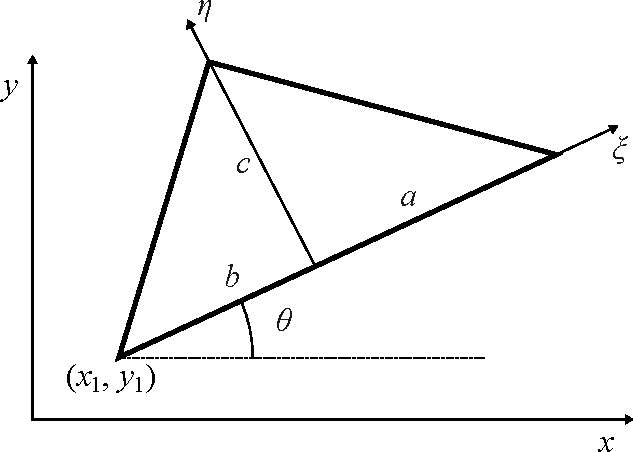
\includegraphics{figures/C1_element.pdf}
\caption{\label{fig:C1}The geometry of a mesh element in the toroidal plane\cite{Jardin04}}
\end{center}
\end{figure}

\paragraph{\texttt{mesh/elements}} is a 2D array consisting of
\texttt{nelms} rows (one per mesh element), with 8 (for 2D
simulations) or 10 (for 3D simulations) columns:

\[ a, b, c, \theta, x_1, y_1, \text{ibound}, \text{izone}, d, \varphi_1 \]

The first five columns ($a$ through $y_1$) describe the geometry of
the element in the toroidal plane, as illustrated in
figure~\ref{fig:C1}.  $d$ and $\varphi_1$ represent the toroidal
extent of the element and the toroidal coordinate of the first
bounding plane (in radians if itor=1, in units of $L_0$ otherwise),
and are only present for 3D simulations.

\paragraph{Fields/} is a group containing the field data.  Each field
is a 2D array consisting of \texttt{nelms} rows (one per element) and
20 (in 2D) or 80 (in 3D) columns, representing the coefficients of
each shape function within the given mesh element.

The field $\phi$ at the coordinate system $(\xi,\eta,\zeta)$ local to the mesh element is given by
\[ 
  \phi(\xi,\eta,\zeta) = \sum_{j=0}^{J} \sum_{i=1}^{20} a_{i + 4(j-1)} \xi^{m_i} \eta^{n_i} \zeta^j
\]
where
\begin{eqnarray*}
   m & = & \{0,1,0,2,1,0,3,2,1,0,4,3,2,1,0,5,3,2,1,0 \}\\
   n & = & \{0,0,1,0,1,2,0,1,2,3,0,1,2,3,4,0,2,3,4,5 \}\\
\end{eqnarray*}
and where $J=3$ for 3D simulations and $J=0$ for 2D / complex simulations.

The fields that are written include the following.  (Note that in 2D
complex simulations, these field names contain the real part of the
field data; for each field an additional field with the suffix "\_i"
is written to contain the imaginary part.)

\begin{tabular}{llll}
\textbf{Field} & \textbf{Units (itor=1)} & \textbf{Units (itor=0)} & \textbf{Description}\\
\hline
psi  & $B_0 L_0^2$ & $B_0 L_0$   & $\psi$\\
I    & $B_0 L_0$   & $B_0$       & $F$ \\
f    & $B_0 L_0$   & $B_0 L_0^2$ & $f$ \\
phi  & $v_0$       & $v_0 L_0$   & $U$ \\
V    & $v_0/L_0$   & $v_0$       & $\omega$ \\
chi  & $v_0 L_0^3$ & $v_0 L_0$   & $\chi$ \\
P    & $p_0$       & $p_0$       & $p$ \\
Pe   & $p_0$       & $p_0$       & $p_e$ \\
ti   & $T_0$       & $T_0$       & $T_i$ \\
te   & $T_0$       & $T_0$       & $T_e$ \\
den  & $n_0$       & $n_0$       & $n_i$ \\
ne   & $n_0$       & $n_0$       & $n_e$
\end{tabular}



\include{physics_model}

\chapter{Boundary Conditions}

In all cases, $f = 0$ on the boundary, and therefore also $\uvec{t}
\cdot \grad{f} = 0$.  Some other boundary conditions that may be
specified are as follows:

\begin{description}
\item[No normal flow (\texttt{inonormalflow=1})] Holds $\uvec{n} \cdot
  \u$ constant.
\item[No poloidal flow (\texttt{inoslip\_pol=1})] Holds $\uvec{t} \cdot
  \u$ constant.
\item[No toroidal flow (\texttt{inoslip\_tor=1})] Holds $\uvec{\tor}
  \cdot \u$ constant.
\item[No normal current (\texttt{inocurrent\_norm=1})] Holds $\uvec{n} \cdot
  \j$ constant.
\item[No poloidal current (\texttt{inocurrent\_pol=1})] Holds $\uvec{t} \cdot
  \j$ constant.
\item[No toroidal current (\texttt{inocurrent\_tor=1})] Holds $\uvec{\tor}
  \cdot \j$ constant.
\end{description}

\begin{eqnarray}
  \uvec{n} \cdot \u & = & 
  -R \uvec{t}\cdot\grad{U}+ \frac{1}{R^2} \uvec{n} \cdot \grad{\chi}
  \\
  \uvec{t} \cdot \u & = & 
  R \uvec{n}\cdot\grad{U} + \frac{1}{R^2} \uvec{t} \cdot \grad{\chi}
  \\
  \uvec{\tor} \cdot \u & = & R \omega
\end{eqnarray}

\begin{eqnarray}
  \uvec{n} \cdot \B & = & 
  -\frac{1}{R} \uvec{t}\cdot\grad{\psi}
  - \frac{1}{R^2} \uvec{n} \cdot \grad{f_\tor}
  \\
  \uvec{t} \cdot \B & = & 
  \frac{1}{R} \uvec{n}\cdot\grad{\psi} 
  \\
  \uvec{\tor} \cdot \B & = & \frac{F}{R}
\end{eqnarray}

\begin{eqnarray}
  \uvec{n} \cdot \j & = & 
  -\frac{1}{R} \uvec{t} \cdot \grad{F}
  + \frac{1}{R^2} \uvec{n} \cdot \grad{\psi_\tor}
  \\
  \uvec{t} \cdot \j & = & 
  \frac{1}{R} \uvec{n}\cdot\grad{(F + f_{\tor \tor})} 
  + \frac{1}{R^2} \uvec{t} \cdot \grad{\psi_\tor}
  \\
  \uvec{\tor} \cdot \j & = & -\frac{1}{R}\gs{\psi}
\end{eqnarray}
In the above definitions, $\uvec{n}$ is the unit vector normal to the
boundary surface, and $\uvec{t} = \uvec{\tor} \times \uvec{n}$.

\section{Resistive Wall Boundary Condition}

For a thin resistive wall of resistivity $\eta_W$ and width
$\delta_W$, the following equations are obtained at the
boundary~\cite{Jardin10}:
\begin{eqnarray}
  \ddt{\psi} & = & -\frac{\eta_W}{\delta_W} \left(\uvec{n} \cdot
  \grad{\psi} - R \uvec{t} \cdot \B_v \right)
    \\
  \ddt{F} & = & -\frac{\eta_W}{\delta_W} \left(F - R \uvec{\tor} \cdot
  \B_v \right)
\end{eqnarray}
Here, $\B_v$ is the magnetic field on the outside of the wall.  $B_v$
may be obtained from the magnetic field on the inside of the wall
using a vacuum response matrix calculated by the $\textsc{vacuum}$
code,~\cite{Chance10} for example.

\subsection{Using a resistive wall in \codename\ with \textsc{vacuum}}

The following assumes that the \textsc{vacuum} code is located in the
directory \texttt{\$VACUUM\_DIR}.  On \texttt{sunfire},
\texttt{\$VACUUM\_DIR = /u/chance/Vacuum\_SVN\_Work}

\begin{enumerate}
\item Build \textsc{struct2vac} with\\
  \texttt{make OPT=1 struct2vac}
\item Generate \texttt{ordered.points} by running \textsc{struct2vac}
  in the working directory.
\item \texttt{tac ordered.points > vacin\_c1}
\item Edit \texttt{vacin\_c1}, and move the last line to be the first
  line.
\item \texttt{cp vacin\_c1 ordered.points}
\item \texttt{cp \$VACUUM\_DIR/Runs/C1Vac/modiv\_m3dc1 .}
\item \texttt{\$VACUUM\_DIR/Bin/vacuum.x86\_64.linux vacin\_c1 modiv\_m3dc1}
\item In \texttt{C1input}, set \texttt{eta\_wall} and
  \texttt{delta\_wall} to the appropriate values.
\end{enumerate}

Presently, the resistive wall only works on single-process runs.



\chapter{Discretization}

\section{Finite Elements}

Each field is represented as a linear combination of $N$ basis
functions $\nu_i$ on the computational domain
\[ U = \sum_{i=1}^N \nu_i U_i. \]
The finite element used in \codename is the reduced quintic element
\cite{Jardin04}, in which the basis functions are fifth order
polynomials.  At each time step, the projection of the equations onto
the basis functions are computed and solved.  For example, the
equation
\[ \ddt{U} = F(U) \]
becomes the system of projection equations
\[ \int dV\, \nu_i \ddt{U} = \int dV\, \nu_i F(U). \]
These projections equations are known collectively as the \emph{weak
form} of the equation.  Solving the equation in this manner is known
as the \emph{Galerkin method}.  Hereafter the index $i$ will be
dropped from $\nu_i$.

Once the equations are cast in the weak form, integrations by parts
may be carried out in order to reduce the order of the differential
operators acting on the physical fields.  For example, 
\begin{eqnarray*}
  \int dV\, \nu \nabla^2 U 
  & = & \int dV\, \div{(\nu \grad{U})} - \grad{\nu} \cdot \grad{U}\\
  & = & \oint d\vec{A} \cdot \grad{U} \nu - \int dV\, \ip{\nu}{\nabla U}\\
  & = & - \int dV\, \ip{\nu}{U}.
\end{eqnarray*}
It is found that using integrations by parts to re-cast the equations
into a form in which a roughly equal number of derivatives acts on the
trial function as on the physical fields improves the numerical
stability of methods for solving the equations.  Thus, in the above
example, the form $-\ip{\nu}{U}$ is preferable to $\nu \nabla^2
U$.

\subsection{Weak form of Physical Equations}

\subsubsection{Integration Identities}

Rather than performing integrations by parts directly on each term in
equations~(\ref{eq:scalar_equations}), it is simpler to begin directly
from the vector form, equations~(\ref{eq:xmhd}) and use the following
identities when applying the operations to extract the scalar
equations:
\begin{eqnarray*}
  -\int dV\, R^2 \nu \grad{\tor} \cdot \curl{\vec{A}} & = & 
  -\int dV\, \vec{A} \cdot \left[\grad{(R^2 \nu)} \times \grad{\tor}
    \right]
  \\
  \int dV\, \nu \div{\vec{A}} & = & 
  -\int dV\, \grad{\nu} \cdot \vec{A}.
\end{eqnarray*}
(Note that the torodal operator, $R^2 \nu \grad{\tor} \cdot$, is not a
differential operator and therefore the integration by parts cannot be
performed \emph{a priori}.)  

Similary, useful identities for the operators that will act on the
stress tensor $\P$ are:
\begin{subequations}
\label{eq:tensor_identities}
\begin{eqnarray}
  R^2 \nu \grad{\tor} \cdot \curl{(\div{\P})} & = & 
  R^2 \partial_Z \nu \grad{\tor} \cdot \P \cdot \grad{\tor}
  - \grad{\nu} \cdot \P \cdot \grad{Z}
  \\ && \mbox{}
  + r \grad{\tor} \cdot \left[\grad{\grad{(\nu r)}} \dottimes \P\right]
  + \div{ \vec{A}_1 }\nonumber
  \\
  -R^2 \nu \grad{\tor} \cdot (\div{\P}) & = &
  R^2 \grad{\nu} \cdot \P \cdot \grad{\tor}
  + \div{\vec{A}_2}
  \\
  -\nu \div{(\div{\P})} & = & -\grad{\grad{\nu}} \dotdot \P + \div{\vec{A}_3}
\end{eqnarray}
\end{subequations}
where
\begin{eqnarray*} 
  \vec{A}_1 & = & 
  - R^2 \nu \grad{\tor} \times (\div{\P})
  - r \P \cdot \left[ \grad{\tor} \times \grad{(r \nu)} \right]
  + \nu \P \cdot \grad{Z}
  \\
  \vec{A}_2 & = & -R^2 \nu \P \cdot \grad{\tor}
  \\
  \vec{A}_3 & = & \grad{\nu} \cdot \P - \nu \div{\P}.
\end{eqnarray*}
(These identities hold for any symmetric tensor $\P$.)  The total
divergences vanish upon integration.

\subsection{Physical Equations after Integrations by Parts}

\begin{subequations}
  \label{eq:equations_ibp}
\begin{eqnarray}
  \int dV\, N_n & = & \int dV\, \left[
    N_{n U} + N_{n \chi} + N_{n D} \right]
  \\
  \int dV\, \left[U_{U n} + U_{\chi n}\right] & = & \int dV\, 
  \left[ 
    U_{U U n} + U_{V V n} + U_{U \chi n} + U_{\chi \chi n} 
    \right. \\ && \nonumber \left. \mbox{} 
    + U_{\psi \psi} + U_{F F} + U_{U \mu} + U_{\chi \mu} + U_g
    \right. \\ && \nonumber \left. \mbox{} 
    + U_{U D} + U_{\chi D} + U_{\P_\parallel} + U_{\P_\times}
    \right]
  \\
  \int dV\, V_{V n} & = & \int dV\, \left[
    V_{V U n} + V_{V \chi n} + V_{\psi F} + V_{V \mu} 
    \right. \\ && \nonumber \left. \mbox{} + V_{V D}  
    + V_{\P_\parallel} + V_{\P_\times} \right]
  \\
  \int dV\, \left[X_{U n} + X_{\chi n}\right] & = & \int dV\, \left[
    X_{U U n}+ X_{V V n}+ X_{U \chi n}+ X_{\chi \chi n} 
    \right.\\  && \nonumber \left. \mbox{} 
    + X_p + X_{\psi \psi} + X_{F F} + X_{U \mu} + X_{\chi \mu} + X_g 
    \right. \\ && \nonumber \left. \mbox{} 
    + X_{U D} + X_{\chi D} + X_{\P_\parallel} + X_{\P_\times}
    \right]
  \\
  \int dV\, \Psi_\psi & = & \int dV\, \left[
    \Psi_{\psi U} + \Psi_{\psi \chi} + \Psi_{\psi F n}
    + \Psi_{\psi \eta} \right]
  \\
  \int dV\, F_F & = & \int dV\, \left[
    F_{F U} + F_{\psi V} + F_{F \chi} + F_{\psi n} + F_{F n} 
    \right. \\ && \nonumber \left. \mbox{} + F_{p_e n} + F_{F \eta} \right]
  \\
  \int dV\, P_p & = & \int dV\, \left[
    P_{p U} + P_{p \chi} + P_{p_e F n} + P_{\eta \psi} + P_{\eta F} 
    \right. \\ && \nonumber \left. \mbox{} 
    + P_\kappa + P_{\kappa_\parallel} + P_{\kappa_\times} \right]
\end{eqnarray}
\end{subequations}

The terms in the above equations are categorized and defined in the
following sections.  Each term has been integrated by parts to arrive
at the simplest expression having for which the order of
differentiation on the trial function is roughly equal to that on the
physical fields.

\subsubsection{Basic Terms}

The terms in this section are the basic terms in the two-fluid
equations, which do not depend on any specific choice of closure.

\begin{equation}
  \begin{array}{ll}
  N_n(\nu, \dot{n}) & = \nu \dot{n}\\
  N_{n U}(\nu, n, U) & = \nu \pb{U}{n}\\
  N_{n \chi}(\nu, n, \chi) & = n \ip{\nu}{\chi}\\
  N_{n D}(\nu, n, D) & = - D \ip{\nu}{n}
  \end{array}
\end{equation}

\begin{equation}
  \begin{array}{lcl}
    U_{U n}(\nu, \dot U, n) & = & -\frac{1}{R^2} n \ip{R^2 \nu}{\dot{U}}
    \\
    U_{\chi n}(\nu, \dot \chi, n) & = & -R^2 \nu \pb{n}{\dot{\chi}}
    \\
    U_{U U n}(\nu, U, U, n) & = & \frac{1}{R^2} n \gs{U} \pb{R^2\nu}{U}
      + \frac{1}{2 R^2} \ip{U}{U}\pb{R^2\nu}{n}
    \\
    U_{V V n}(\nu, V,  V, n) & = &  \frac{1}{2 R^2} \pb{\nu}{R^2} V V n
    \\
    U_{U \chi n}(\nu, U, \chi, n) & = & 
      \frac{1}{R^2}n \gs{U}\ip{R^2\nu}{\chi} 
      - \pb{U}{\chi} \pb{R^2\nu}{n}
    \\
    U_{\chi \chi n}(\nu, \chi, \chi, n) & = &
      \frac{1}{2} \ip{\chi}{\chi} \pb{R^2 \nu}{n}
    \\
    U_{\psi \psi}(\nu, \psi, \psi) & = &
      -\frac{1}{R^2} \pb{R^2 \nu}{\psi} \gs{\psi}
    \\
    U_{F F}(\nu, F, F) & = & -R^2 \nu F \pb{F}{\frac{1}{R^2}}
    \\
    U_{U D}(\nu, U, D) & = & \frac{1}{R^2} \ip{R^2 \nu}{U} D
    \\
    U_{\chi D}(\nu, \chi, D) & = & -\pb{R^2 \nu}{\chi} D
  \end{array}
\end{equation}

\begin{equation}
  \begin{array}{lcl}
    V_{V n}(\nu, V, n) & = & \nu n \dot{V}\\
    V_{V U n}(\nu, V, U, n) & = & \nu n \pb{U}{V}\\
    V_{V \chi n}(\nu, V, \chi, n) & = & -\nu n \ip{\chi}{V}\\
    V_{\psi F}(\nu, \psi, F) & = & \nu \pb{F}{\psi}\\
    V_{V D}(\nu, V, D) & = & -\nu V D
  \end{array}
\end{equation}    

\begin{equation}
  \begin{array}{lcl}
    X_{U n}(\nu, \dot U, n) & = & \nu \pb{n}{\dot{U}}
    \\
    X_{\chi n}(\nu, \dot \chi, n) & = & -n \ip{\nu}{\dot{\chi}}
    \\
    X_p(\nu, p) & = & \ip{\nu}{p}
    \\
    X_{U U n}(\nu, U, U, n) & = & -\frac{1}{R^2} n \gs{U} \ip{\nu}{U}
      + \frac{1}{2} n \ip{\nu}{\frac{\ip{U}{U}}{R^2}}
    \\
    X_{V V n}(\nu, V,  V, n) & = & 
      \frac{1}{2} n V V \ip{\frac{1}{R^2}}{\nu}
    \\
    X_{U \chi n}(\nu, U, \chi, n) & = & 
      \left( n \lp{\nu} + \ip{n}{\nu} \right) \pb{U}{\chi}
      + n \gs{U} \pb{\nu}{\chi}
    \\
    X_{\chi \chi n}(\nu, \chi, \chi, n) & = & \frac{1}{2} n 
      \ip{\nu}{\ip{\chi}{\chi}}
    \\
    X_{\psi \psi}(\nu, \psi, \psi) & = & 
      \frac{1}{R^2} \gs{\psi} \ip{\nu}{\psi}
    \\
    X_{F F}(\nu, F, F) & = & \frac{1}{R^2} F \ip{\nu}{F}
    \\
    X_{U D}(\nu, U, D) & = & \pb{\nu}{U} D
    \\
    X_{\chi D}(\nu, \chi, D) & = & \ip{\nu}{\chi} D
  \end{array}
\end{equation}


\begin{equation}
  \begin{array}{lcl}
    \Psi_{\psi}(\nu, \dot{\psi}) & = & \nu \dot{\psi}\\
    \Psi_{\psi U}(\nu, \psi, U) & = & \nu \pb{U}{\psi}\\
    \Psi_{\psi \chi}(\nu, \psi, \chi) & = & -\nu \ip{\chi}{\psi}\\
    \Psi_{\psi F n}(\nu, \psi, F, n) & = & d_i \nu \frac{1}{n} \pb{\psi}{F}\\
    \Psi_{\psi \eta}(\nu, \psi, \eta) & = & 
        -\frac{1}{R^2} \ip{\psi}{R^2 \nu \eta} 
  \end{array}
\end{equation}

\begin{equation}
  \begin{array}{lcl}
    F_F (\nu, \dot{F}) & = & \nu \dot{F}\\
    F_{F U}(\nu, F, U) & = & R^2 \nu \pb{U}{\frac{F}{R^2}}\\
    F_{\psi V}(\nu, \psi, V) & = & R^2 \nu \pb{\frac{V}{R^2}}{\psi}\\
    F_{F \chi}(\nu, F, \chi) & = & \frac{F}{R^2} \ip{R^2 \nu}{\chi}\\
    F_{\psi n}(\nu, \psi, \psi, n) & = &
       d_i \frac{\gs{\psi}}{R^2 n}\pb{\psi}{R^2\nu}\\
    F_{F n}(\nu, F, F, n) & = &
       d_i R^2 \nu F \pb{\frac{1}{R^2 n}}{F}\\
    F_{p_e n}(\nu, p_e, n) & = & d_i R^2 \nu \pb{\frac{1}{n}}{p_e}\\
    F_{F \eta}(\nu, F, \eta) & = & -\frac{1}{R^2} \eta \ip{R^2 \nu}{F}
  \end{array}
\end{equation}

\begin{equation}
  \begin{array}{lcl}
  P_p(\nu, \dot{p}) & = & \nu \dot{p}
  \\
  P_{p U}(\nu, p, U) & = & \nu \pb{U}{p}
  \\
  P_{p \chi}(\nu, p, \chi) & = & \Gamma p \ip{\nu}{\chi} 
    + (\Gamma - 1) \nu \ip{p}{\chi}
  \\
  P_{p_e, F, n}(\nu, p_e, F, n) & = & d_i \left( 
      \frac{1}{n} \nu \pb{p_e}{F} 
    + \Gamma \nu p_e \pb{\frac{1}{n}}{F} \right)
  \\
  P_{\eta, \psi}(\nu, \eta, \psi, \psi) & = & (\Gamma - 1) \nu
  \frac{(\gs{\psi})^2}{R^2}
  \\
  P_{\eta, F}(\nu, \eta, F, F) & = & (\Gamma - 1) \nu \frac{F^2}{R^2}
  \end{array}
\end{equation}

\subsubsection{Gravity}

These terms are obtained assuming a gravitational force of the form given by
equation~(\ref{eq:gravity}).

\begin{equation}
  \begin{array}{lcl}
    U_g(\nu, n) & = & g_r \nu \pb{n}{R} - g_Z r \nu \ip{n}{R}
    \\
    X_g(\nu, n) & = & \frac{n}{R^2} \left( 
    g_r \ip{\nu}{R} + g_Z r \pb{\nu}{R} \right)
  \end{array}
\end{equation}



\subsubsection{Heat Flux Terms}

These terms are obtained assuming a heat flux density of the form
described in section~\ref{sec:heat_flux}.

\begin{equation}
  \begin{array}{lcl}
    P_\kappa(\nu, \kappa, T) & = &
    -(\Gamma - 1) \kappa \ip{\nu}{T}
    \\
    P_{\kappa_\parallel}(\nu, \kappa_\parallel, T, \psi, \psi, B^{-2}) & = &
    -(\Gamma - 1) \kappa_\parallel \frac{1}{B^2} \pb{\psi}{\nu} \pb{\psi}{T}
    \\
    P_{\kappa_\times}(\nu, \kappa_\times, T, F, B^{-2}) & = & 
    (\Gamma - 1) \kappa_\times \frac{F}{B} \pb{\nu}{T}
  \end{array}
\end{equation}

\begin{eqnarray*}
  T & = & p/n \\
  B^2 & = & \frac{1}{R^2} \left[ \ip{\psi}{\psi} + F^2 \right]
\end{eqnarray*}


\subsubsection{Isotropic Viscosity}

These terms result from isotropic viscosity of the form given by
equation~(\ref{eq:general_viscosity}).

\begin{equation}
  \begin{array}{lcl}
    U_{U \mu}(\nu, U, \mu) & = & \frac{1}{R^2} \left [ \left(
      \ip{\mu}{R^2 \nu} + \mu \gs{(R^2 \nu)} \right) \gs{U} \right. \\
      & & \left. \mbox{} + \lp{\mu} \ip{R^2 \nu}{U} 
      + \gs{(R^2 \nu)} \ip{\mu}{U} \right]
    \\
    U_{\chi \mu}(\nu, \chi, \mu) & = & -\lp{(R^2 \nu)} \pb{\mu}{\chi}
      - \gs{\mu}\pb{R^2\nu}{\chi} \\ & & \mbox{}
      - \frac{1}{R^2}\gs{(R^2 \chi)} \pb{R^2 \nu}{\mu}
    \\
    V_{V \mu}(\nu, V, \mu) & = & \left[\ip{\nu}{\mu} 
      + \frac{1}{R^2}\mu \gs{(R^2 \nu)} \right] V
    \\
    X_{U \mu}(\nu, U, \mu) & = & \lp{\nu} \pb{\mu}{U} 
      + \lp{\mu} \pb{\nu}{U} + \gs{U} \pb{\nu}{\mu}
    \\
    X_{\chi \mu}(\nu, \chi, \mu, \mu_c) & = & 
      \lp{\nu} \ip{\mu}{\chi} + \lp{\mu} \ip{\nu}{\chi}
      + 2 \mu_c \lp{\nu} \lp{\chi}
  \end{array}
\end{equation}

\subsubsection{Parallel Viscosity}

These terms are obtained assuming a parallel viscosity of the form
given in equation~(\ref{eq:parallel_viscosity}).  These equations were
obtained using equations~(\ref{eq:tensor_identities}).  For
compactness, derivatives are written as subscripts in the following
expressions (\textit{i.e.} $\nu_Z = \partial_Z \nu$).

\begin{equation}
  \begin{array}{lcl}
    U_{\P_\parallel U}(\nu, U) & = & {\mu_\parallel}_U D_U
    \\
    U_{\P_\parallel V}(\nu, V) & = & {\mu_\parallel}_V D_U
    \\
    U_{\P_\parallel \chi}(\nu, \chi) & = & {\mu_\parallel}_\chi D_U
  \end{array}
\end{equation}

\begin{equation}
  \begin{array}{lcl}
    V_{\P_\parallel U}(\nu, U) & = & {\mu_\parallel}_U D_V
    \\
    V_{\P_\parallel V}(\nu, V) & = & {\mu_\parallel}_V D_V
    \\
    V_{\P_\parallel \chi}(\nu, \chi) & = & {\mu_\parallel}_\chi D_V
  \end{array}
\end{equation}

\begin{equation}
  \begin{array}{lcl}
    X_{\P_\parallel U}(\nu, U) & = & {\mu_\parallel}_U D_X
    \\
    X_{\P_\parallel V}(\nu, V) & = & {\mu_\parallel}_V D_X
    \\
    X_{\P_\parallel \chi}(\nu, \chi) & = & {\mu_\parallel}_\chi D_X
  \end{array}
\end{equation}

\begin{eqnarray*}
  D_U & = & \frac{3}{B^2} \left\{ 
  - \frac{1}{2}R^2\pb{\nu}{\frac{\ip{\psi}{\psi}}{R^2}}
  + \ip{\psi}{\pb{\nu}{\psi}} 
  - \frac{1}{R^2} F^2 \nu_Z 
  \right.\\ && \left. \mbox{}
  - \frac{2}{R^2}\left[ \nu_Z (\psi_Z^2 - \psi_R^2) + 2\nu_r \psi_r \psi_Z
    \right]
  \right\}
  \\
  D_V & = & - 3 \frac{F}{B^2} \pb{\nu}{\psi}
  \\
  D_X & = & - \lp{\nu} 
  \left(1 - \frac{3}{R^2}\frac{\ip{\psi}{\psi}}{B^2} \right)
  \\ &&  \mbox{}
  + \frac{3}{R^2 B^2} \left(
    \frac{1}{2}R^2\ip{\nu}{\frac{\ip{\psi}{\psi}}{R^2}}
    - \ip{\psi}{\ip{\nu}{\psi}} 
    + \frac{1}{R} F^2 \nu_r \right)
\end{eqnarray*}

\begin{eqnarray*}
  {\mu_\parallel}_U & = & \eta_0 \frac{p_i \tau_i}{R^2 B^2} \left( 
  - \frac{1}{2} R^2 \pb{U}{\frac{\ip{\psi}{\psi}}{R^2}}
  + \ip{\psi}{\pb{U}{\psi}}
  - \frac{1}{R^2} F^2 U_Z \right)
  \\
  {\mu_\parallel}_V & = & -\eta_0 p_i \tau_i \frac{F}{B^2} 
  \pb{\psi}{\frac{V}{R^2}}
  \\
  {\mu_\parallel}_\chi & = & \eta_0 \frac{p_i \tau_i}{R^2 B^2} \left(
    \frac{1}{2} R^2 \ip{\chi}{\frac{\ip{\psi}{\psi}}{R^2}}
  - \ip{\psi}{\ip{\chi}{\psi}}
  + \frac{1}{R} F^2 \chi_r 
  \right.\\ && \left. \mbox{}
  + \lp{\chi} \ip{\psi}{\psi}
  \right)
\end{eqnarray*}


\subsubsection{Gyroviscosity}

These terms are obtained using equations~(\ref{eq:tensor_identities})
assuming a gyroviscosity of the form given by
equation~(\ref{eq:gyroviscosity}).

\begin{eqnarray*}
  & \lefteqn{U_{\P_\times U}(\nu, U) = -\frac{p_i F}{2 R^3 B^2}} & 
  \\ & & \mbox{} \times
    \left\{ \begin{array}{l} 
      \left(1+\frac{3}{2 R^2}\frac{\ip{\psi}{\psi}}{B^2}\right)
      \left[ \begin{array}{r@{}l}
	     & \left( [R^3 \nu_Z]_Z - [R^3 \nu_r]_r \right)
	       \left( \left[\frac{U_R}{R}\right]_Z 
	            + \left[\frac{U_Z}{R}\right]_r \right) 
             \\ \mbox{}
	   - & \left( [R^3 \nu_r]_Z + [R^3 \nu_Z]_r \right)
	       \left( \left[\frac{U_Z}{R}\right]_Z 
	            - \left[\frac{U_R}{R}\right]_r \right) 
	     \end{array} \right]
       \\ \mbox{}
      + \frac{9}{2 r B^2} 
      \\ \mbox{} \times \left[ 
	\begin{array}{r@{}l}
	  \left( \psi_Z^2 - \psi_R^2 \right) &
	  \left( r \nu_Z \left[ 
	    \left( \frac{U_Z}{R} \right)_Z -
	    \left( \frac{U_R}{R} \right)_r \right]
          -\frac{1}{R^3} U_Z \left[ 
	    (R^3 \nu_Z)_Z - (R^3 \nu_r)_r \right] \right)
	  \\ 
	  \mbox{} + 2 \psi_r \psi_Z &
          \left( r \nu_Z \left[ 
	    \left( \frac{U_R}{R} \right)_Z +
	    \left( \frac{U_Z}{R} \right)_r \right]
          -\frac{1}{R^3} U_Z \left[ 
	    (R^3 \nu_r)_Z + (R^3 \nu_Z)_r \right] \right)
	  \end{array} \right] 
    \end{array} \right\}
\end{eqnarray*}

\begin{eqnarray*}
  & \lefteqn{U_{\P_\times V}(\nu, V) = -\frac{p_i}{B^2}} &
  \\ && \mbox{} \times
  \left\{ \begin{array}{l}
      \frac{1}{4 R^2} \left(1 - \frac{3 F^2}{B^2 R^2} \right) 
      \\ \mbox{} \times
      \left( \ip{\frac{V}{R^2}}{R^4 \pb{\psi}{\nu}}
            -\ip{\psi}{R^4\pb{\nu}{\frac{V}{R^2}}}
	    +\frac{1}{R^2}\pb{\nu}{R^6\ip{\frac{V}{R^2}}{\psi}} \right)
      \\ \mbox{}
      -\frac{3}{4 B^2} \pb{\psi}{\frac{V}{R^2}}
      \\ \mbox{} \times
      \left( 2 \ip{\psi}{\ip{\psi}{\nu}}
           - R^2 \ip{\nu}{\frac{\ip{\psi}{\psi}}{R^2}}
	   - \gs{\nu} \ip{\psi}{\psi}
	   + 6 \psi_Z \pb{\nu}{\psi} \right)
      \\ \mbox{}
      +\frac{9 F^2}{2 B^2 R^2} \nu_Z \ip{\psi}{\frac{V}{R^2}}
    \end{array} \right\}
\end{eqnarray*}

\begin{eqnarray*}
  & \lefteqn{U_{\P_\times \chi}(\nu, \chi) = -\frac{p_i F}{2 R^3 B^2}} &
  \\ && \mbox{} \times 
  \left\{ \begin{array}{l}
    \left[ \left( \chi_{R R} - \chi_{Z Z} \right)
           \left( [R^3 \nu_r]_r - [R^3 \nu_Z]_Z \right)
       +   2 \chi_{R Z} 
           \left( [R^3 \nu_r]_Z + [R^3 \nu_Z]_r \right)
           \right]
    \\ \mbox{}
    + \frac{3}{R^2 B^2} \left[ \begin{array}{l} 
	\left( \gs{\chi}[\psi_Z^2 - \psi_R^2] 
        - \chi_{Z Z} \psi_Z^2 + \chi_{R R} \psi_R^2 \right)
	\left( [R^3 \nu_r]_r - [R^3 \nu_Z]_Z \right)
	\\ \mbox{} + 2 \chi_{R Z} 
	\left( \psi_Z^2 [R^3 \nu_r]_Z
	      +\psi_R^2 [R^3 \nu_Z]_r \right)
	\\ \mbox{} - 2 \psi_r \psi_Z 
	\left( \left[\chi_{Z Z} - \frac{1}{R}\chi_r \right] [R^3 \nu_r]_Z
	      +\left[\chi_{R R} - \frac{1}{R}\chi_r \right][R^3 \nu_Z]_r 
	      \right)
      \end{array} \right]
  \end{array} \right\}
\end{eqnarray*}

\begin{eqnarray*}
  & \lefteqn{V_{\P_\times U}(\nu, U) = \frac{p_i}{4 r B^2}} &
  \\ && \mbox{} \times 
  \left\{ \begin{array}{l}
    \left(1 - \frac{3}{R^2} \frac{F^2}{B^2} \right)
    \left( \ip{\psi}{R \pb{U}{\nu}}+\ip{\nu}{R \pb{U}{\psi}}
          -\frac{1}{R^3} \pb{U}{R^4 \ip{\nu}{\psi}}
	  +U_r \pb{\nu}{\psi} + \frac{2}{R} \psi_Z \ip{\nu}{U} \right)
    \\ \mbox{} + 
    \frac{3}{R B^2} \pb{\psi}{\nu}
    \left( 2\ip{\psi}{\ip{U}{\psi}} - \gs{U}\ip{\psi}{\psi} 
          - \frac{1}{R^2}\ip{U}{R^2\ip{\psi}{\psi}} 
	  +\pb{\psi}{R^2}\pb{\psi}{U} \right)
    \\ \mbox{} - 
    \frac{18}{R^2} \frac{F^2}{B^2} \pb{U}{R} \ip{\nu}{\psi}
  \end{array} \right\}
\end{eqnarray*}

\begin{eqnarray*}
  V_{\P_\times V}(\nu, V) & = & \frac{p_i F R^2}{4 B^2}
  \left(1 - \frac{3}{R^2} \frac{\ip{\psi}{\psi} - F^2}{B^2} \right)
    \pb{\nu}{\frac{V}{R^2}}
\end{eqnarray*}

\begin{eqnarray*}
  & \lefteqn{V_{\P_\times \chi}(\nu, \chi) = \frac{p_i}{B^2}} &
  \\ && \mbox{} \times 
  \left\{ \begin{array}{l}
    \left( \frac{1}{R^2}\ip{\chi}{R^2 \ip{\nu}{\psi}}
          -\ip{\nu}{\ip{\chi}{\psi}} - \ip{\psi}{\ip{\nu}{\chi}} \right)
    \\ \mbox{} + \frac{3}{2 r B^2} \pb{\psi}{\nu}
    \left( \ip{\psi}{R \pb{\chi}{\psi}} 
         - \frac{1}{2} r \pb{\chi}{\ip{\psi}{\psi}} \right)
    \\ \mbox{} + \frac{3}{4 R^2} \frac{F^2}{B^2}
    \left( \ip{\psi}{\ip{\chi}{\nu}} + \ip{\nu}{\ip{\chi}{\psi}}
          -\ip{\chi}{\ip{\nu}{\psi}} - 2 \gs{\chi}\ip{\nu}{\psi} \right)
  \end{array} \right\}
\end{eqnarray*}

\begin{eqnarray*}
  & \lefteqn{X_{\P_\times U}(\nu, U) = \frac{p_i F}{2 R^2 B^2}} &
  \\ && \mbox{} \times  
  \left\{ \begin{array}{l}
  \funcss{\nu}{U} - R^2 \funcaa{\nu}{U} 
  + \frac{1}{R} \left[ U_r (\nu_{Z Z} - \nu_{R R})
                     -2 U_Z \nu_{R Z} - \frac{1}{R} U_r \nu_r \right]
  \\ \mbox{}
  + \frac{3}{R B^2} \left[ \begin{array}{l}
    \left( \left[\frac{U_Z}{R} \right]_Z 
         - \left[\frac{U_R}{R} \right]_r \right)
    \left(\nu_{Z Z} \psi_R^2 - \nu_{R R} \psi_Z^2
         +\frac{1}{R} \nu_r [\psi_Z^2 - \psi_R^2] \right)
    \\ \mbox{}
    + 2\nu_{R Z} \left( 
        \left[ \frac{U_R}{R} \right]_Z \psi_R^2
      + \left[ \frac{U_Z}{R} \right]_r \psi_Z^2
      - \frac{1}{R^2} U_Z [\psi_Z^2 - \psi_R^2] \right)
    \\ \mbox{}
    - 2 \psi_r \psi_Z \left( \begin{array}{l}
        \left[ \frac{U_R}{R} \right]_Z \nu_{R R}
      + \left[ \frac{U_Z}{R} \right]_r \nu_{Z Z}
      - \frac{1}{R^2} U_Z [\nu_{Z Z} - \nu_{R R}] 
      \\ \mbox{}
      - \frac{1}{R} \nu_r \left[ 
	  \left( \frac{U_R}{R} \right)_Z
	+ \left( \frac{U_Z}{R} \right)_r \right] 
      \end{array} \right)
    \end{array} \right]
  \end{array} \right\}
\end{eqnarray*}

\begin{eqnarray*}
  & \lefteqn{X_{\P_\times V}(\nu, V) = \frac{p_i}{4 B^2}} &
  \\ && \mbox{} \times 
  \left\{ \begin{array}{l}
    \left(1 - \frac{3}{R^2} \frac{F^2}{B^2} \right) \left(
    \frac{1}{R^2} \ip{\nu}{R^2\ip{\frac{V}{R^2}}{\psi}}
    - \ip{\psi}{\ip{\frac{V}{R^2}}{\nu}}
    - \ip{\frac{V}{R^2}}{\ip{\psi}{\nu}} \right)
    \\ \mbox{} + \frac{6}{B^2} \pb{\psi}{\frac{V}{R^2}}
    \left(\frac{1}{R} \ip{\psi}{R \pb{\nu}{\psi}}
    - \frac{1}{2} \pb{\nu}{\ip{\psi}{\psi}} \right)
    \\ \mbox{} - 6 \frac{F^2}{B^2} \ip{\psi}{\frac{V}{R^2}}
    \left[ \left(\frac{\nu_Z}{R^2} \right)_Z
         + \left(\frac{\nu_R}{R^2} \right)_r \right]
  \end{array} \right\}
\end{eqnarray*}


\begin{eqnarray*}
  & \lefteqn{X_{\P_\times \chi}(\nu, \chi) = -\frac{p_i F}{B^2}} &
  \\ && \mbox{} \times 
  \left\{ \begin{array}{l}
    \left(1 + \frac{3}{2 R^2} \frac{\ip{\psi}{\psi}}{B^2} \right)
    \funcsa{\nu}{\chi}
    \\ \mbox{} + \frac{3}{2 B^2} \left[ \begin{array}{r@{}l}
      & \left(- \frac{1}{2} \pb{\chi}{\ip{\psi}{\psi}}
	      + \frac{1}{R} \ip{\psi}{R\pb{\chi}{\psi}} 
             \right)
	\left( \left[ \frac{\nu_R}{R^2} \right]_r
	     + \left[ \frac{\nu_Z}{R^2} \right]_Z \right)
    \\ \mbox{}
     - & \left(- \frac{1}{2} \pb{\nu}{\ip{\psi}{\psi}}
               + \frac{1}{R} \ip{\psi}{R\pb{\nu}{\psi}} 
              \right)
         \left( \left[ \frac{\chi_R}{R^2} \right]_r
	      + \left[ \frac{\chi_Z}{R^2} \right]_Z \right)
      \end{array} \right]
  \end{array} \right\}
\end{eqnarray*}

\subsection{Spatial Integration}

The integrals required to calculate the weak-form equations of the
Galerkin method are computed numerically using a 79-point Gaussian
quadrature.  That is, the value of each field is calculated at 79
points for each triangular element, and a weighted sum of these values
is computed to approximate the integral.
\[
  \int dA\ f(x) \simeq \sum_{i=1}^{79} w_i f(x_i),
\]
where the integrand $f(x)$ is restricted to a single element.  The
sampling points and weights appropriate for a equilateral triangle are
taken from ref.~\cite{Dunavant85}.

The coordinates of the sampling points are given in the ``natural
coordinates'' $(\alpha, \beta, \gamma)$ in ref.~\cite{Dunavant85}.
These coordinates may be converted to cartesian coordinates $(r, Z)$
for an equilateral triangle $e$ having vertices
\[
\left\{\left(-\frac{\sqrt{3}}{2},-\frac{1}{2}\right),
\left(\frac{\sqrt{3}}{2},-\frac{1}{2}\right), (0,1)\right\} 
\]
using the linear transformation
\[ 
\phi_{n \to e}(\alpha, \beta, \gamma) = 
\left(\frac{\sqrt{3}}{2}(\beta-\gamma), \frac{1}{2}(3 \alpha - 1)
\right).
\]
The weights must be multiplied by the Jacobian of this transformation,
\[
\mathcal{J}_{\phi_{n \to e}} = \frac{3 \sqrt{3}}{4}.
\]
To find the coordinates of the sampling points for a general triangle
$g$ having vertices $\{(-b,0), (a,0), (0,c)\}$, as in
ref.~\cite{Jardin04}, one may use the linear transformation
\begin{eqnarray*}
  \phi_{e \to g}(r,Z) & = & 
    \left(\frac{a+b}{\sqrt{3}} x + \frac{a-b}{3} (1-y), 
    \frac{c}{3}(2y+1) \right) \\
  \mathcal{J}_{\phi_{e \to g}} & = &  \frac{2 c}{3 \sqrt{3}} (a+b).
\end{eqnarray*}
The transformation from natural coordinates to cartesian coordinates
for a triangle having vertices $\{(-b,0), (a,0), (0,c)\}$ is therefore
\begin{eqnarray*}
  \phi_{n \to g}(r,Z) & = & 
  \left(\frac{1}{2} (a+b) (\beta-\gamma) +
  \frac{1}{2} (a-b)(1-\alpha), c \alpha \right) \\
  \mathcal{J}_{\phi_{n \to g}} & = & \frac{1}{2} (a+b) c.
\end{eqnarray*}

The 79-point quadrature gives the exact results for integrands which
are polynomials of degree 20 (or less).  In the case of quintic finite
elements, this means the integration is exact for terms involving
products of three fields or fewer, not including the degree-five
trial function $\nu$.  In cylindrical geometry, the presence factors
of $1/R$ will cause the quadrature not to be exact, as $1/R$ is not in
the form of a polynomial.  The weights $w_i$ must also be multiplied
by $R_i$ in cylindrical coordinates to account for the Jacobian of the
transformation from cartesian to cylindrical coordinates.


\section{Time step}



\subsection{Implicit Time Advance}

For the implicit time advance, equations~(\ref{eq:equations_ibp}) are
evaulated at the $\theta$-advanced time (\emph{e.g.} $F(\psi) \to
F(\psi + \theta \dt \dot{\psi} + \cdots)$), linearized (\emph{i.e.}
$\order{\dt^2}$ and higher are dropped), and then discretized
temporally according to the chosen time integration method
(\emph{i.e.} $\dot{\psi} \to (\psi^{(n+1)} - \psi^{(n)})/\dt$).


\begin{eqnarray}
  \begin{pmatrix}
    \cola{S^v_{1 1}} & \cola{R^v_{1 1}} &
    \colb{S^v_{1 2}} & \colb{R^v_{1 2}} & 
          S^v_{1 3}  &        0         &
          R^v_{1 4}  &       R^v_{1 3}
    \\
    \cola{R^B_{1 1}} & \cola{S^B_{1 1}} &
    \colb{R^B_{1 2}} & \colb{S^B_{1 2}} & 
          R^B_{1 3}  &       S^B_{1 3}  &
              0      &        0
    \\
    \colb{S^v_{2 1}} & \colb{R^v_{2 1}} & 
    \colb{S^v_{2 2}} & \colb{R^v_{2 2}} & 
          S^v_{2 3}  &        0         &
	  R^v_{2 4}  &       R^v_{2 3}
    \\
    \colb{R^B_{2 1}} & \colb{S^B_{2 1}} &
    \colb{R^B_{2 2}} & \colb{S^B_{2 2}} & 
          R^B_{2 3}  &       S^B_{2 3}  &
              0      &        0
    \\
          S^v_{3 1}  &       R^v_{3 1}  &
          S^v_{3 2}  &       R^v_{3 2}  &
          S^v_{3 3}  &        0         &
	  R^v_{3 4}  &       R^v_{3 3}  
    \\
          R^B_{3 1}  &       S^v_{3 1}  &
          R^B_{3 2}  &       S^v_{3 2}  &
          R^B_{3 3}  &       S^v_{3 3}  &
              0      &        0
    \\
          R^n_{3 1}  &        0         &
          R^n_{3 2}  &        0         &
          R^n_{3 3}  &        0         &
          S^n        &        0
    \\
          R^p_{3 1}  &        0         &
          R^p_{3 2}  &        0         &
          R^p_{3 3}  &        0         &
              0      &       S^p        &
  \end{pmatrix}
  \begin{pmatrix}
    \cola{U}\\ \cola{\psi}\\ 
    \colb{V}\\ \colb{F}   \\
    \chi \\ p_e \\ 
    n \\ p
  \end{pmatrix}^{(n+1)} = \nonumber \\
  \begin{pmatrix}
    \cola{D^v_{1 1}} & \cola{Q^v_{1 1}} &
    \colb{D^v_{1 2}} & \colb{Q^v_{1 2}} & 
          D^v_{1 3}  &        0         &
          Q^v_{1 4}  &       Q^v_{1 3}
    \\
    \cola{Q^B_{1 1}} & \cola{D^B_{1 1}} &
    \colb{Q^B_{1 2}} & \colb{D^B_{1 2}} & 
          Q^B_{1 3}  &       D^B_{1 3}  &
              0      &        0
    \\
    \colb{D^v_{2 1}} & \colb{Q^v_{2 1}} & 
    \colb{D^v_{2 2}} & \colb{Q^v_{2 2}} & 
          D^v_{2 3}  &        0         &
	  Q^v_{2 4}  &       Q^v_{2 3}
    \\
    \colb{Q^B_{2 1}} & \colb{D^B_{2 1}} &
    \colb{Q^B_{2 2}} & \colb{D^B_{2 2}} & 
          Q^B_{2 3}  &       D^B_{2 3}  &
              0      &        0
    \\
          D^v_{3 1}  &       Q^v_{3 1}  &
          D^v_{3 2}  &       Q^v_{3 2}  &
          D^v_{3 3}  &        0         &
	  Q^v_{3 4}  &       Q^v_{3 3}  
    \\
          Q^B_{3 1}  &       D^v_{3 1}  &
          Q^B_{3 2}  &       D^v_{3 2}  &
          Q^B_{3 3}  &       D^v_{3 3}  &
              0      &        0
    \\
          Q^n_{3 1}  &        0         &
          Q^n_{3 2}  &        0         &
          Q^n_{3 3}  &        0         &
          D^n        &        0
    \\
          Q^p_{3 1}  &        0         &
          Q^p_{3 2}  &        0         &
          Q^p_{3 3}  &        0         &
              0      &       D^p        &
  \end{pmatrix}
  \begin{pmatrix}
    \cola{U}\\ \cola{\psi}\\ 
    \colb{V}\\ \colb{F}   \\
    \chi \\ p_e \\ 
    n \\ p
  \end{pmatrix}^{(n)} +   
  \begin{pmatrix}
    Q_1 \\ Q_2 \\ 
    Q_3 \\ Q_4 \\
    Q_5 \\ Q_6 \\ 
    Q_7 \\ Q_8
  \end{pmatrix}
\end{eqnarray}

\subsection{Split Time Step Method}



Time is advanced using a split time-step method in which the velocity
field is advanced first, then the density and total pressure fields
are advanced separately, and finally the magnetic field and electron
pressure are advanced together.  Though the velocity and magnetic
field are advanced separately, the Alfv\'en and magnetosonic waves are
treated implicitly by using
equations~(\ref{eq:scalar_p}--\ref{eq:scalar_F}) to calculate
analytically the advanced-time values of the pressure and magnetic
field for use in the velocity time step.



\begin{eqnarray}
  \label{eq:velocity_advance}
  \lefteqn{
  \begin{pmatrix}
    \cola{S^v_{1 1}} & \colb{S^v_{1 2}} & S^v_{1 3}\\
    \colb{S^v_{2 1}} & \colb{S^v_{2 2}} & S^v_{2 3}\\
          S^v_{3 1}  &       S^v_{3 2}  & S^v_{3 3}\\
  \end{pmatrix} 
  \begin{pmatrix}
    \cola{U}\\ \colb{V}\\ \chi
  \end{pmatrix}^{(n+1)}}\\
  & = & 
  \begin{pmatrix}
    \cola{D^v_{1 1}} & \colb{D^v_{1 2}} & D^v_{1 3}\\
    \colb{D^v_{2 1}} & \colb{D^v_{2 2}} & D^v_{2 3}\\
          D^v_{3 1}  &       D^v_{3 2}  & D^v_{3 3}\\
  \end{pmatrix} 
  \begin{pmatrix}
    \cola{U}\\ \colb{V}\\ \chi
  \end{pmatrix}^{(n)}
  + 
  \begin{pmatrix}
    \cola{Q^v_{1 1}} & \colb{Q^v_{1 2}} & Q^v_{1 3}\\
    \colb{Q^v_{2 1}} & \colb{Q^v_{2 2}} & Q^v_{2 3}\\
          Q^v_{3 1}  &       Q^v_{3 2}  & Q^v_{3 3}\\
  \end{pmatrix} 
  \begin{pmatrix}
    \cola{\psi}\\ \colb{F}\\ p
  \end{pmatrix}^{(n)} \nonumber
  \\ & & \mbox{} + 
  \begin{pmatrix}
    \cola{O^v_{1}}\\
    \colb{O^v_{2}}\\
          O^v_{3} \\
  \end{pmatrix} \nonumber
\end{eqnarray}

\begin{eqnarray}
  \label{eq:density_advance}
  S^n n^{(n+1)} & = & D^n n^{(n)} + 
  \begin{pmatrix} R^n_1 & R^n_2 & R^n_3\end{pmatrix}
  \begin{pmatrix}\cola{U}\\ \colb{V}\\ \chi\end{pmatrix}^{(n+1)}
  \\ & & \mbox{} + 
  \begin{pmatrix}Q^n_1    &   Q^n_2   & Q^n_3\end{pmatrix}
  \begin{pmatrix}\cola{U}\\ \colb{V}\\ \chi\end{pmatrix}^{(n)} \nonumber
\end{eqnarray}


\begin{eqnarray}
  \label{eq:pressure_advance}
  S^p p^{(n+1)} & = & D^p p^{(n)} + 
  \begin{pmatrix}R^p_1 & R^p_2 & R^p_3\end{pmatrix}
  \begin{pmatrix}\cola{U}\\ \colb{V}\\ \chi \end{pmatrix}^{(n+1)}
  \\ & & \mbox{} + 
  \begin{pmatrix}Q^p_1 & Q^p_2 & Q^p_3\end{pmatrix}
  \begin{pmatrix}\cola{U}\\ \colb{V}\\ \chi \end{pmatrix}^{(n)} \nonumber
\end{eqnarray}


\begin{eqnarray}
  \label{eq:field_advance}
  \lefteqn{
  \begin{pmatrix}
    \cola{S^B_{1 1}} & \colb{S^B_{1 2}} & S^B_{1 3}\\
    \colb{S^B_{2 1}} & \colb{S^B_{2 2}} & S^B_{2 3}\\
          S^B_{3 1}  &       S^B_{3 2}  & S^B_{3 3}\\
  \end{pmatrix} 
  \begin{pmatrix}
    \cola{\psi}\\ \colb{F}\\ p_e
  \end{pmatrix}^{(n+1)}}\\
  & = & 
  \begin{pmatrix}
    \cola{D^B_{1 1}} & \colb{D^B_{1 2}} & D^B_{1 3}\\
    \colb{D^B_{2 1}} & \colb{D^B_{2 2}} & D^B_{2 3}\\
          D^B_{3 1}  &       D^B_{3 2}  & D^B_{3 3}\\
  \end{pmatrix} 
  \begin{pmatrix}
    \cola{\psi}\\ \colb{F}\\ p_e
  \end{pmatrix}^{(n)} +
  \begin{pmatrix}
    \cola{R^B_{1 1}} & \colb{R^B_{1 2}} & R^B_{1 3}\\
    \colb{R^B_{2 1}} & \colb{R^B_{2 2}} & R^B_{2 3}\\
          R^B_{3 1}  &       R^B_{3 2}  & R^B_{3 3}\\
  \end{pmatrix} 
  \begin{pmatrix}
    \cola{U}\\ \colb{V}\\ \chi
  \end{pmatrix}^{(n+1)} \nonumber
  \\ & & \mbox{} +
  \begin{pmatrix}
    \cola{Q^B_{1 1}} & \colb{Q^B_{1 2}} & Q^B_{1 3}\\
    \colb{Q^B_{2 1}} & \colb{Q^B_{2 2}} & Q^B_{2 3}\\
          Q^B_{3 1}  &       Q^B_{3 2}  & Q^B_{3 3}\\
  \end{pmatrix} 
  \begin{pmatrix}
    \cola{U}\\ \colb{V}\\ \chi
  \end{pmatrix}^{(n)} +
  \begin{pmatrix}
    \cola{O^B_{1}}\\
    \colb{O^B_{2}}\\
          O^B_{3} \\
  \end{pmatrix} \nonumber
\end{eqnarray}

\subsubsection{Linear Calculations}

Linear calculations may be performed by calculating each matrix once,
and recalculating the matrix-vector products each time step with the
updated vectors.  This method is very efficient because the $S$
matrices need only be inverted once, and in all subsequent time steps
the only matrix operations carried out are addition and matrix-vector
multiplication.  Non-linear simulations require all the matrices to be
recalculated each time step, and the $S$ matrices must be inverted
each time step.

\subsubsection{Implementation of Electron Pressure Equation}

Because it is the electron pressure which appears in the generalized
Ohm's law, equation~(\ref{eq:ohm}), if the electron pressure equation
is retained, it is solved with the magnetic field as the third row in
equation~(\ref{eq:field_advance}) so as to keep the fast magnetosonic
wave implicit.  In this case, the full pressure is evolved
independently in equation~(\ref{eq:pressure_advance}).  If the
electron pressure equation is not included, the third row in
equation~(\ref{eq:field_advance}) is the total pressure equation, and
the electron pressure is assumed to remain always at a specific
fraction of the total pressure, which is determined by the initial
conditions.


\subsection{Crank-Nicholson}

The Crank-Nicholson time step is defined by the following discretization:
\begin{eqnarray*}
  \frac{\partial U}{\partial t} & \to & 
  \frac{U^{(n+1)} - U^{(n)}}{\dt}\\
  U & \to & \thimp U^{(n+1)} + (1-\thimp) U^{(n)}.
\end{eqnarray*}
By Taylor expanding about $U$,
\begin{eqnarray*}
  U^{(n+1)} & = & U + \thimp\,\dt\,\dot{U} + \frac{1}{2} \thimp^2 \dt^2
  \ddot{U} + \frac{1}{6} \thimp^3 \dt^3 \dddot{U}+ \cdots
  \\
  U^{(n)} & = & U + (\thimp-1) \dt\, \dot{U} + \frac{1}{2} (\thimp-1)^2 \dt^2
  \ddot{U} + \frac{1}{6} (\thimp-1)^3 \dt^3 \dddot{U} + \cdots
\end{eqnarray*}
the trunctation error of the time-derivative operator can be
calculated directly:
\begin{eqnarray*}
  \Delta_{CN}(\dt, \thimp) & = & \frac{U^{(n+1)} - U^{(n)}}{\dt} -
 \dot{U}
 \\ 
 & = & 
  \left( \thimp-\frac{1}{2} \right) \dt\,\ddot{U}
  + \frac{1}{2} \left(\thimp^2 - \thimp + \frac{1}{3} \right) \dt^2 \dddot{U}
  + \cdots.
\end{eqnarray*}
When $\thimp=1/2$, the time differencing is ``time-centered'' because
the two points involved in the time differencing are equidistant in
the logical time coordinate from the point at which the field itself
is evaluated.  In this case, the leading-order truncation error is
$\order{\dt^2}$:
\begin{equation}
  \Delta_{CN}(\dt, \thimp=1/2) = \frac{1}{24} \dt^2 \dddot{U} + \cdots.
\end{equation}

\subsection{BDF2}

The BDF2 time step is defined by the following discretization:
\begin{eqnarray*}
  \frac{\partial U}{\partial t} & \to & 
  \frac{3 U^{(n+1)} - 4 U^{(n)} + U^{(n-1)}}{2\,\dt}\\
  U & \to & U^{(n+1)}.
\end{eqnarray*}
Taylor expanding about $U$:
\begin{eqnarray*}
  U^{(n+1)} & = & U
  \\
  U^{(n)} & = & U - \dt\, \dot{U} + \frac{1}{2} \dt^2 \ddot{U} 
  - \frac{1}{6} \dt^3 \dddot{U} + \cdots
  \\
  U^{(n-1)} & = & U - 2\,\dt\, \dot{U} + 2\,\dt^2 \ddot{U} 
  - \frac{4}{3} \dt^3 \dddot{U} + \cdots
\end{eqnarray*}
and the truncation error is
\begin{equation}
  \Delta_{BDF2}(\dt) = 
  \frac{3 U^{(n+1)} - 4 U^{(n)} + U^{(n-1)}}{2\,\dt} - \dot{U} = 
  - \frac{1}{3} \dt^2 \dddot{U}
  + \cdots.
\end{equation}


\chapter{Input Parameters}
\label{sec:input_parameters}

\subsection{Model Options}

\begin{tabular}{llp{3in}}
  \textbf{Option}&\textbf{Default}&\textbf{Description}\\
  \hline
  \texttt{numvar} & 3   & MHD model. 1: 2-field;  2: 4-Field;  3: 6-Field.\\
  \texttt{idens}  & 1   & 1: include density equation\\
  \texttt{ipres}  & 0   & 1: include electron pressure equation\\
  \texttt{gyro}   & 0   & 1: include gyroviscous term\\
  \texttt{itor}   & 0   & 0: cartesian; 1: cylindrical\\
  \texttt{linear} & 0   & 1: linear (perturbation terms only, no matrix
                              recalculation)\\
  \texttt{eqsubtract}& 0& 1: remove equilibrium terms from equations\\
  \texttt{isource}   & 0& 1: include ``source'' terms in velocity
    advance\\
  \texttt{igauge} & 0   & 1: Loop voltage appears explicitly in Ohm's law.\\
  \texttt{ntor}   & 0   & The toroidal modenumber of linear perturbations in
                          complex simulations.\\
  \texttt{istatic}& 0   & 1: Do not advance velocity\\
  \texttt{iestatic}&0   & 1: Do not advance magnetic fields\\
  \texttt{inertia} & 1  & 1: Include $\u \cdot \grad{\u}$ terms\\
  \texttt{itwofluid}& 1 & 1: Include $\j\times\B$ and
  $\grad{p_e}$ terms in Ohm's law\\ 
\end{tabular}


\subsection{Physical Parameters}

\begin{tabular}{llcl}
  \textbf{Option}&\textbf{Var.}&\textbf{Default}&\textbf{Description}\\
  \hline
  \texttt{gam}    & $\Gamma$& 5/3 & Adiabatic constant\\
  \texttt{db}     & $d_i$   & 0   & Ion skin depth\\
  \texttt{gravr}, \texttt{gravz} & \vec{g} & 0 & \parbox[t]{1.8in}{Gravity.\\
                       $\vec{g} = -(\mathtt{gravr}/R^2) \uvec{R} 
                                  - \mathtt{gravz}\ \uvec{Z}$.}
\end{tabular}


\subsection{Transport Coefficients}

\begin{tabular}{llcp{2.25in}}
  \textbf{Option}&\textbf{Var.}&\textbf{Default}&\textbf{Description}\\
  \hline
  \texttt{denm}      & $D_n$   & 0   & Density diffusion coefficient\\
  \hline
  \texttt{amu}       & $\mu_r$       & 0 & \\
  \texttt{amu\_edge} & $\mu_0$       & 0 & \\
  \texttt{amuoff}    & $\Psi_c^\mu$ & 0 & \\
  \texttt{amudelt}   & $\Delta^\mu$ & 0 & \\
  \texttt{iresfunc} & & 0 &
  \begin{minipage}[t]{2.2in}
    0: $\mu = \mu_r$\\
    2: $\mu = \mu_r + \frac{1}{2}\mu_0 \{1 + \tanh[(\Psi - \Psi_c^{\mu})/\Delta^{\mu}]\}$\\
    3: $\mu = \mu_r + \eta_0 H(\Psi - \Psi_c^{\mu})$\\
  \end{minipage}\\  
  \texttt{amuc}   & $\mu_c$ & $\mu_r$ & Compressional viscosity coefficient\\
  \texttt{amupar} & $\mu_\parallel$ & 0 & Parallel viscosity coefficient\\
  \hline
  \texttt{etar}   & $\eta_r$   & 0 & \\
  \texttt{eta0}   & $\eta_0$ & 0 & \\
  \texttt{etaoff} & $\Psi_c^\eta$ & 0 & \\
  \texttt{etadelt}& $\Delta^\eta$ & 0 & \\
  \texttt{iresfunc} & & 0 &
  \begin{minipage}[t]{2.2in}
    0: $\eta = \eta_r + \eta_0/T_e^{3/2}$\\
    2: $\eta = \eta_r + \frac{1}{2}\eta_0 \{1 + \tanh[(\Psi - \Psi_c^{\eta})/\Delta^{\eta}]\}$\\
    3: $\eta = \eta_r + \eta_0 H(\Psi - \Psi_c^{\eta})$\\
    4: $\eta = \eta_{Spitzer}$
  \end{minipage}\\
  \hline
  \texttt{kappat}   & $\eta_t$    & 0 & \\
  \texttt{kappa0}   & $\eta_0$    & 0 & \\
  \texttt{kappaoff} & $\Psi_c^\kappa$ & 0 & \\
  \texttt{kappadelt}& $\Delta^\kappa$ & 0 & \\
  \texttt{iresfunc} & & 0 &
  \begin{minipage}[t]{2.2in}
    0: $\kappa = \kappa_t + \kappa_0*p/T^{3/2}$\\
    2: $\kappa = \kappa_t + \frac{1}{2}\kappa_0 \{1 + \tanh[(\Psi - \Psi_c^{\kappa})/\Delta^{\kappa}]\}$
  \end{minipage}\\
  \texttt{kappar} & $\kappa_\parallel$ & 0 
                  & Parallel thermal conductivity\\
  \texttt{ikapscale}& & 0 & 1: Multiply \texttt{kappar} by $\kappa$\\
  \texttt{kappax} & $\kappa_\times$ & 0 
                  & Crosswise thermal conductivity\\ 
\end{tabular}

\subsection{Hyper-Diffusivity}

\begin{tabular}{lcp{2.2in}}
  \textbf{Option} & \textbf{Default} & \textbf{Description}\\
  \hline
  \texttt{xzero}  & 0 & $R$-coordinate of bottom left corner of domain\\
  \texttt{zzero}  & 0 & $Z$-coordinate of bottom left corder of domain\\
  \texttt{iper}   & 0 & 1: Left/right boundaries periodic\\
  \texttt{jper}   & 0 & 2: Top/bottom boundaries periodic\\
  \texttt{inonormalflow}& 1 & 1: No-normal-flow boundary\\
  \texttt{inoslip\_pol} & 0 & 1: No-slip boundaries for poloidal velocity\\
  \texttt{inoslip\_tor} & 1 & 1: No-slip boundaries for toroidal velocity\\
  \texttt{inostress\_tor}&0 & 1: No-normal-stress boundary for toroidal 
                                 velocity\\
  \texttt{com\_bc}& 1 & 1: $\nabla^2 \chi = 0$\\
  \texttt{iconst\_t}  & 0 & 0: $\partial_t T = 0$\\
  \texttt{inograd\_t} & 0 & 0: No normal temperature gradient\\
  \texttt{vloop}  & 0 & Loop voltage.  $\partial_t \psi = \mathtt{vloop}$\\
  \texttt{imask}  & 0 & 1: Smoothly bring $d_i$ to zero near
    boundaries\\
  \texttt{amu\_edge} & 0 &    Factor by which to increase viscosity near 
                              boundaries
\end{tabular}


\subsection{Time Integration Options}
\begin{tabular}{lcp{3in}}
  \textbf{Option}&\textbf{Default}&\textbf{Description}\\
  \hline
  \texttt{dt}         & 0.1 & Time step\\
  \texttt{ntimemax}   & 20  & Total number of time steps\\
  \texttt{integrator} & 0   & 0: Crank-Nicholson (CN); 1: BDF2\\
  \texttt{imp\_mod}   & 0   & 
  \begin{minipage}[t]{3in}
    0: $\theta$-implicit\\
    1: Implicit leapfrof (\texttt{isplitstep} = 1 only)\\
  \end{minipage}\\
  \texttt{thimp}      & 0.5 & Implicitness parameter\\
  \texttt{thimp\_ohm} & \texttt{thimp} & 
                              Implicitness of ohmic heating terms\\
  \texttt{thimpsm}    & 1   & Implicitness of the smoother functions\\
  \texttt{isplitstep} & 1   & 0: Fully implicit time step; 
                              1: split time step.\\
  \texttt{iresolve}   & 0   & 1: Re-solve velocity after 
                              field advance of split time step.\\
  \texttt{iteratephi} & 0   & 1: Calculate transport coefficients after
    field advance, then recalculate field advance.
\end{tabular}


\subsection{Spatial Integration Options}
\begin{tabular}{lcp{3in}}
  \textbf{Option}&\textbf{Default}&\textbf{Description}\\
  \hline
  \texttt{int\_pts\_main}  & 79 & Sampling points for integrations in
                                main time step matrices\\
  \texttt{int\_pts\_aux}   & 79 & Sampling points for integrations in
                                calculations of auxiliary variables\\
  \texttt{int\_pts\_diag}  & 79 & Sampling points for integrations in
                                diagnostic calculations\\
\end{tabular}


\subsection{Numerical Options}
\begin{tabular}{llp{3in}}
  \textbf{Option}&\textbf{Default}&\textbf{Description}\\
  \hline
  \texttt{ivform} & 0   & 0: $\u = \grad{U}\times\grad{\tor} + V
   \grad{\tor} + \grad{\chi}$\\
   & & 1: $\u = \r^2 \grad{U}\times\grad{\tor} + \r^2 \omega
   \grad{\tor} + \r^{-2} \grad{\chi}$\\
  \texttt{jadv}   & 0   & 1: Use toroidal current density equation
                          instead of poloidal flux equation.\\
  \texttt{max\_ke}& 1.0  & Maximum value of kinetic energy before solution is
                          rescaled in linear simulations. (0 = don't rescale)\\
  \texttt{harned\_mikic} & 0.0 & Coefficient of Harned-Mikic two-fluid
                          stabilization term.\\
\end{tabular}

\subsection{Input/Output Options}

\begin{tabular}{lcp{2.7in}}
  \textbf{Option}&\textbf{Default}&\textbf{Description}\\
  \hline
  \texttt{ntimepr}   & 5 & Number of timesteps per full field output\\
  \texttt{iprint}    & 0 & 1: Print detailed info to stdout\\
  \texttt{iglobalout}& 0 & 1: Write process-independent output file\\
  \texttt{iglobalin} & 0 & 1: Read process-independent output file on restart\\
  \texttt{irestart}  & 0 & 1: Read restart file\\
  \texttt{iread\_eqdsk}   & 0 & 1: Read EFIT g-file 'geqdsk'\\
  \texttt{iread\_dskbal}  & 0 & 1: Read BAL file 'dskbal'\\
  \texttt{iread\_jsolver} & 0 & 1: Read Jsolver file 'fixed'
\end{tabular}


\subsection{Initial Conditions Options}

\begin{tabular}{llcp{2.5in}}
  \textbf{Option}&\textbf{Var.}&\textbf{Default}&\textbf{Description}\\
  \hline
  \texttt{itaylor} & & 0 & \begin{minipage}[t]{2.5in}
    Pre-defined initial conditions.\\
    0: Tilting cylinder\\
    1: Taylor Reconnection\\
    2: Force-Free equilibrium\\
    3: GEM Reconnection\\
    4: Wave Propagation\\
    5: Gravitational Instability\\
  \end{minipage}\\
  \texttt{irmp} & & 0 & 
  \begin{minipage}[t]{2.5in}
    Add nonaxisymmetric perturbation from
    \texttt{rmp\_coil.dat} and \texttt{rmp\_current.dat} with $n =
    \mathtt{ntor}$\\
    1: Initial perturbation is vacuum field\\
    2: Perturbation only at boundary
  \end{minipage}\\
  \texttt{maxn}     & & 200 & Maximum wavenumber of initial random noise\\
  \texttt{eps}      & & 0.01 & Size of random perturbation\\
  \texttt{iflip}    & & 0 & 1: Flip coordinate system handedness\\
  \texttt{iflip\_b} & & 0 & 1: Flip sign of toroidal field\\
  \texttt{iflip\_v} & & 0 & 1: Flip sign of toroidal velocity\\
  \texttt{icsym}    & & 0 &
  \begin{minipage}[t]{2.5in}
    Impose symmetry on random perturbations
    0: No symmetry\\
    1: Odd up-down symmetry (in $U$)\\
    2: Even up-down symmetry (in $U$)
  \end{minipage}\\
  \texttt{bscale}      & & 1.0 & Bateman scaling for toroidal field\\
  \hline
  \texttt{den\_edge}   & $\rho_e$      & 0.0 & \\
  \texttt{den0}        & $\rho_0$      & 1.0 & \\
  \texttt{denoff}      & $\Psi_c^\rho$ & 1.0 & \\
  \texttt{dendelt}     & $\Delta^\rho$ & 0.1 & \\
  \texttt{idenfunc}    &               & 0   &
  \begin{minipage}[t]{2.5in}
    0: Use problem-specific density\\
    2: $\rho = \rho_0 + \frac{1}{2}\rho_e \{1 + \tanh[(\Psi - \Psi_c^{\rho})/\Delta^{\rho}]\}$\\
    3: $\rho = \rho_0 + \rho_e H(\Psi - \Psi_c^{\rho})$\\
    4: Read density profile from 'PROFDEN.txt'
  \end{minipage}
\end{tabular}

\subsection{Grad-Shafranov Solver Options}
\begin{tabular}{lcp{3in}}
  \textbf{Option}&\textbf{Default}&\textbf{Description}\\
  \hline
  \texttt{igs}   & 80     & Number of Picard iterations\\
  \texttt{xmag}  & \texttt{xzero}+1 & $R$-coordinate of magnetic axis\\
  \texttt{zmag}  & 0      & $Z$-coordinate of magnetic axis\\
  \texttt{xlim}  & \texttt{xzero}   & $R$-coordinate of limiter\\
  \texttt{zlim}  & 0      & $Z$-coordinate of limiter\\
  \hline
  \texttt{divertors} & 0  & Number of divertors (0--2)\\
  \texttt{divcur}& 0.1    & Divertor current(s), as fraction of tcuro\\
  \texttt{xdiv}  & 0      & $r$-coordinate of divertor current(s)\\
  \texttt{zdiv}  & 0      & \parbox[t]{3in}{$z$-coordinate of 
    divertor 
    current.  If $\mathtt{divertors} = 2$, the second divertor has 
    $z = -\mathtt{zdiv}$.}\\
  \hline
  \texttt{tcuro} & 1      & Plasma current in GS equilibrium\\
  \texttt{q0}    & 1      & Safety factor at magnetic axis\\
  \texttt{djdpsi}& 0      & $J_\tor'(\Psi)$ at magnetic axis\\
  \texttt{bzero} & 1      & $B_\tor$ at \texttt{rzero}\\
  \texttt{pedge} & 0      & Pressure in vacuum region\\
  \texttt{p0}    & 0.01   & Pressure at magnetic axis\\
  \texttt{p1}    & -1     & $p'(\Psi)$ at magnetic axis\\
  \texttt{p2}    & -2     & $p''(\Psi)$ at magnetic axis\\
  \texttt{pedge} & 0      & Pressure in vacuum region\\
  \texttt{divertors} & 0  & Number of divertors (0--2)\\
  \texttt{divcur}& 0.1    & Divertor current(s), as fraction of tcuro\\
  \texttt{xdiv}  & \texttt{xmag} & $R$-coordinate of divertor current(s)\\
  \texttt{zdiv}  & \texttt{zmag} & \parbox[t]{3in}{$Z$-coordinate of 
    divertor 
    current.  If $\mathtt{divertors} = 2$, the second divertor has 
    $Z = -\mathtt{zdiv}$.}\\
  \texttt{expn}  & 0 & \parbox[t]{3in}{Fraction of pressure gradient due to
    density gradient: $n = p^\mathtt{expn}$.}\\
  \texttt{psiscale} & 1.0 & Rescale profiles s.t. LCFS is at 
  $\Psi=\mathtt{psiscale}$.
\end{tabular}



\subsection{Boundary and Domain Options}

\begin{tabular}{lcp{2.5in}}
  \textbf{Option} & \textbf{Default} & \textbf{Description}\\
  \hline
  \texttt{xzero}  & 0 & $r$-coordinate of bottom left corner of domain\\
  \texttt{zzero}  & 0 & $z$-coordinate of bottom left corder of domain\\
  \texttt{iper}   & 0 & 1: Left/right boundaries periodic\\
  \texttt{jper}   & 0 & 2: Top/bottom boundaries periodic\\
  \hline
  \texttt{ifixedb} & 0 & Set $\psi=0$ on boundary\\
  \texttt{inonormalflow}& 1 & 1: No-normal-flow boundary\\
  \texttt{inoslip\_pol} & 0 & 1: No-slip boundaries for poloidal velocity\\
  \texttt{inoslip\_tor} & 1 & 1: No-slip boundaries for toroidal velocity\\
  \texttt{inostress\_tor}&0 & 1: No-normal-stress boundary for toroidal 
                                 velocity\\
  \texttt{iconst\_bz} & 1 & 1: Toroidal field held constant on boundary\\
  \texttt{iconst\_n}  & 0 & 1: Density held constant on boundary\\
  \texttt{iconst\_p}  & 1 & 1: Pressure held constant on boundary\\
  \texttt{iconst\_t}  & 0 & 1: Temperature held constant on boundary\\
  \texttt{inograd\_p} & 0 & 1: No normal pressure gradient\\
  \texttt{inograd\_t} & 0 & 1: No normal temperature gradient\\
  \texttt{com\_bc}& 0 & 1: $\nabla^2 \chi = 0$\\
  \texttt{vor\_bc}& 0 & 1: $\Delta^* U = 0$\\
  \texttt{imask}  & 0 & 1: Smoothly bring $d_i$ to zero near
    boundaries\\
  \hline
  \texttt{eta\_wall}   & 0 & Resistivity of the wall\\
  \texttt{delta\_wall} & 1 & Thickness of the resistive wall
\end{tabular}



\subsection{Unit Normalizations}
\begin{tabular}{lcp{3in}}
  \textbf{Option}&\textbf{Default}&\textbf{Description}\\
  \hline
  \texttt{n0\_norm} & $10^{14}$ & Density normalization (in cgs)\\
  \texttt{b0\_norm} & $10^4$    & Magnetic field normalization (in cgs)\\
  \texttt{l0\_norm} & $100$     & Length normalization (in cgs)
\end{tabular}


\subsection{Current Controller Options}

\begin{tabular}{llcl}
  \textbf{Option}&\textbf{Var.}&\textbf{Default}&\textbf{Description}\\
  \hline
  \texttt{vloop}      & $V_L$ & 0              & (Initial) loop voltage.\\
  \texttt{tcur}       & $I_0$ & \texttt{tcuro} & Target toroidal current\\
  \texttt{control\_p} & $c_p$ & 0              & Proportional coefficient\\
  \texttt{control\_i} & $c_i$ & 0              & Integral coefficient\\
  \texttt{control\_d} & $c_d$ & 0              & Derivative coefficient\\
\end{tabular}


\subsection{Density Source Options}

\begin{tabular}{llcp{2in}}
  \textbf{Option}&\textbf{Var.}&\textbf{Default}&\textbf{Description}\\
  \hline
  \texttt{ipellet}      & & 0    & 1: include pellet density
    source (\textit{c.f.} section~\ref{sec:pellet_injection})\\
  \texttt{pellet\_rate} & $\alpha_p$ & 0 
                                     & Particle number injection rate\\
  \texttt{pellet\_var}  & $l_p$      & 1    & Variance of  
                                              injection profile\\
  \texttt{pellet\_x}    & $R_p$      & \texttt{xmag} 
                                     & $R$-coordinate of injection profile\\
  \texttt{pellet\_z}    & $Z_p$      & \texttt{zmag} 
                                     & $Z$-coordinate of injection profile\\
  \texttt{ionization}   & & 0  & 1: include neutral ionization
    source (\textit{c.f.} section~\ref{sec:ionization})\\
  \texttt{ionization\_rate} & $\alpha_i$ & 0 
                                     & Ionization rate coefficient\\
  \texttt{ionization\_temp} & $E_i$   & 0.01 & Ionization energy\\
  \texttt{ionization\_depth}& $l_i$   & 0.01 & Temperature 
    scale-length of neutral burn-out
\end{tabular}


\subsection{Diagnostics Options}

\begin{tabular}{lcp{3in}}
  \textbf{Option}&\textbf{Default}&\textbf{Description}\\
  \hline
  \texttt{xnull}     & 0 & Guess for $r$-coordinate of x-point\\
  \texttt{znull}     & 0 & Guess for $z$-coordinate of x-point\\
  \texttt{icalc\_scalars} & 1 & 1: Calculate volume-integrated scalars 
                                (\textit{e.g.} energy)\\
  \texttt{ike\_only} & 0 & 1: Only calculate kinetic energy
\end{tabular}



\bibliographystyle{plain}
\bibliography{doc.bib}

\appendix

\newcommand{\IDLf}[1]{\texttt{\textbf{#1}}}
\newcommand{\IDLa}[1]{\textit{#1}}
\newcommand{\IDLbool}{\texttt{bool}}
\newcommand{\IDLint}{\texttt{int}}
\newcommand{\IDLstr}{\texttt{string}}
\newcommand{\IDLflt}{\texttt{float}}
\newcommand{\IDLopt}[1]{$\langle$ #1 $\rangle$}

\chapter{IDL Postprocessor}


\section{Functions/Procedures in \IDLf{plot\_routines.pro}}

\subsection{Procedure \IDLf{{contour\_and\_legend}}}

\IDLf{{contour\_and\_legend}}, \IDLa{z}, \IDLa{x}, \IDLa{y}

\subsubsection{Description}

This procedure draws a two-dimensional color contour plot of the data
$z$.  \IDLa{nt} frames are drawn.

\subsubsection{Mandatory Arguments}

\begin{tabular}{lcll}
Name & I/O & Type & Description\\
\hline
\IDLa{z} & I & \IDLflt[\IDLa{nt},\IDLa{nx},\IDLa{nz}] 
                                  & The values of the field to plot\\
\IDLa{x} & O & \IDLflt[\IDLa{nx}] & The values of the $x$-coordinate\\ 
\IDLa{y} & O & \IDLflt[\IDLa{nz}] & The values of the $y$-coordinate\\ 
\end{tabular}


\subsubsection{Optional Arguments}

\begin{tabular}{lclp{2.5in}}
Name            & I/O & Type     & Description\\
\hline
\IDLa{label}   & I & \IDLstr[\IDLa{nt}] 
               & The IDL-formatted label of the color bar for each frame\\
\IDLa{title}   & I & \IDLstr[\IDLa{nt}] 
               & The IDL-formatted title of the plot for each frame\\
\IDLa{range}   & I & \IDLflt[2,\IDLa{nt}]
               & An array of the ranges of $z$ to plot in each frame\\
\IDLa{nlevels} & I & \IDLint[\IDLa{nt}] 
               & The number of contour levels to plot for each frame\\
\IDLa{lines}   & I & \IDLbool[\IDLa{nt}]
               & Whether to draw contour lines for each frame\\
\IDLa{zlog}    & I & \IDLbool[\IDLa{nt}]
               & Whether to draw $z$ on a log scale, for each frame\\
\IDLa{jpeg}    & I & \IDLstr
               & Write the resulting .jpeg image to the file \IDLa{jpeg}\\
\IDLa{isotropic}& I & \IDLbool
               & Use an isotropic aspect ratio when plotting\\
\IDLa{color\_table}& I & \IDLint
               & Which intrinsic IDL color table to use when plotting
\end{tabular}





\section{Functions/Procedures in \IDLf{read\_h5.pro}}

\subsection{Function \IDLf{read\_field}}

\IDLf{read\_field}, \IDLa{name}, \IDLa{r}, \IDLa{z}, \IDLa{t}

\subsubsection{Description}

This function reads the raw field data associated with \IDLa{name} in
the specified output file.  The data is interpolated onto a uniform
retangular grid, and returned in an array.

\subsubsection{Return Value}

\IDLflt[\IDLa{nt}, \IDLa{points}, \IDLa{points}] containing the value
of the field at \IDLa{points} $\times$ \IDLa{points} spatial sampling
points at \IDLa{nt} time slices.

\subsubsection{Mandatory Arguments}
\begin{tabular}{lcll}
Name & I/O & Type & Description\\
\hline
\IDLa{name} & I & \IDLstr                & The name of the field to read\\
\IDLa{r}    & O & \IDLflt[\IDLa{points}] & The values of the $r$-coordinate\\ 
\IDLa{z}    & O & \IDLflt[\IDLa{points}] & The values of the $z$-coordinate\\ 
\IDLa{t}    & O & \IDLflt[\IDLa{nt}]     & The values of the $t$-coordinate\\
\end{tabular}

\subsubsection{Optional Arguments}
\begin{tabular}{lclp{2.3in}}
Name            & I/O & Type       & Description\\
\hline
\IDLa{filename} & I   & \IDLstr    
                & The name of the HDF5 file to read\\
\IDLa{points}   & I   & \IDLint
                & Number of sampling points per spatial dimension\\
\IDLa{rrange}   & I   & \IDLflt[2] & Range of $r$-coordinate to read\\
\IDLa{zrange}   & I   & \IDLflt[2] & Range of $z$-coordinate to read\\
\IDLa{h\_symmetry}& I & \IDLopt{1 $|$ -1}
                & Return only left-right \IDLopt{symmetric $|$ anti-symmetric} 
                  part of field\\
\IDLa{v\_symmetry}& I & \IDLopt{1 $|$ -1} 
                & Return only up-down \IDLopt{symmetric $|$ anti-symmetric} 
                  part of field\\
\IDLa{diff}     & I   & \IDLbool   
                & If set, \IDLa{name} should be an array with two filenames.  
                  The difference of the fields from the two files is 
                  returned.\\
\IDLa{slices}   & O   & \IDLopt{\IDLint $|$ \IDLint[2]} 
                & \IDLopt{Time slice $|$ range of~time~slices} to read\\
\IDLa{mesh}     & O   &              & 
\end{tabular}



\subsection{Function \IDLf{flux\_average}}

\IDLf{flux\_average}, \IDLa{field}, \IDLa{slice}

\subsubsection{Description}

This function finds the flux-surface average of the field \IDLa{field}.

\subsubsection{Return Value}

\IDLflt[\IDLa{bins}] containing the value of the flux-averaged field
for a range of values of flux.

\subsubsection{Mandatory Arguments}

\begin{tabular}{lclp{2in}}
Name & I/O & Type & Description\\
\hline
\IDLa{field} & I 
             & \IDLopt{\IDLstr $|$ \IDLflt[1,\IDLa{points},\IDLa{points}]}
             & If \IDLa{field} is type \IDLstr, then read field associated with
               name \IDLa{field}.  Otherwise, \IDLa{field} is taken to contain
               the field data.\\
\IDLa{slice} & I & \IDLint
             & If \IDLa{field} is type \IDLstr, then this is the time slice
               to read.  Otherwise, \IDLa{slice} is ignored.
\end{tabular}

\subsubsection{Optional Arguments}

\IDLf{flux\_average} takes all of the optional arguments for
\IDLf{read\_field}.  In addition, 

\begin{tabular}{lclp{2.5in}}
Name            & I/O & Type       & Description\\
\hline
\IDLa{filename} & I   & \IDLstr    
                & The name of the HDF5 file to read\\
\IDLa{bins}     & I   & \IDLint    
                & Number of bins to subdivide the flux\\
\IDLa{psi}*     & I/O & \IDLflt[1,\IDLa{points},\IDLa{points}]
                & The flux field at the given time slice\\
\IDLa{x}        & I/O & \IDLflt[\IDLa{points}]
                & $r$-coordinate values\\
\IDLa{z}        & I/O & \IDLflt[\IDLa{points}]
                & $z$-coordinate values\\
\IDLa{t}        & I/O & \IDLflt[\IDLa{points}]
                & $t$-coordinate values\\
\IDLa{flux}     & O   & \IDLflt[\IDLa{bins}]
                & The value of the flux for each bin\\
\IDLa{title}    & O   & \IDLstr    
                & The IDL-formatted title of the field\\
\IDLa{symbol}   & O   & \IDLstr     
                & The IDL-formatted symbol of the field\\
\IDLa{units}    & O   & \IDLstr    
                & The IDL-formatted units of the field\\
\end{tabular}
* If \IDLa{psi}, \IDLa{x}, \IDLa{z}, and \IDLa{t} are all provided as
  input, the \IDLf{flux\_average} will not read the flux field itself.




\subsection{Function \IDLf{read\_scalar}}

\IDLf{read\_field}, \IDLa{name}

\subsubsection{Description}

This function reads the scalar quantity associated with \IDLa{name} in
the specified output file.  The data is returned as an array .

\subsubsection{Return Value}

\IDLflt[\IDLa{nt}] containing the value of the scalar at each time
step.

\subsubsection{Mandatory Arguments}

\begin{tabular}{lcll}
Name & I/O & Type & Description\\
\hline
\IDLa{name} & I & \IDLstr                & The name of the scalar to read\\
\end{tabular}

\subsubsection{Optional Arguments}

\begin{tabular}{lcll}
Name            & I/O & Type       & Description\\
\hline
\IDLa{filename} & I   & \IDLstr    & The name of the HDF5 file to read\\
\IDLa{time}     & O   & \IDLflt[\IDLa{nt}] 
                                   & The $t$-coordinate of each element\\
\IDLa{title}    & O   & \IDLstr    & The IDL-formatted title of the scalar\\
\IDLa{symbol}   & O   & \IDLstr    & The IDL-formatted symbol of the scalar\\
\IDLa{units}    & O   & \IDLstr    & The IDL-formatted units of the scalar\\
\end{tabular}





\subsection{Procedure \IDLf{plot\_field}}


\IDLf{plot\_field}, \IDLa{name}, \IDLa{slice}, \IDLa{r}, \IDLa{z}, \IDLa{t}

\subsubsection{Mandatory Arguments}

\begin{tabular}{lcll}
Name & I/O & Type & Description\\
\hline
\IDLa{name} & I & \IDLstr                & The name of the field to read\\
\IDLa{slice} & I & \IDLstr               & The time slice to read\\
\IDLa{r}    & O & \IDLflt[\IDLa{points}] & The values of the $r$-coordinate\\ 
\IDLa{z}    & O & \IDLflt[\IDLa{points}] & The values of the $z$-coordinate\\ 
\IDLa{t}    & O & \IDLflt[\IDLa{nt}]     & The values of the $t$-coordinate\\
\end{tabular}


\subsubsection{Optional Arguments}

\IDLf{plot\_field} takes all of the optional arguments for
\IDLf{read\_field} and \IDLf{contour\_and\_legend}.  In addition, 

\begin{tabular}{lcll}
Name            & I/O & Type       & Description\\
\hline
\IDLa{xrange}   & I   & \IDLflt[2] & Range of $r$-coordinate to plot\\
\IDLa{yrange}   & I   & \IDLflt[2] & Range of $z$-coordinate to plot\\
\IDLa{lcfs}     & I   & \IDLbool   & Plot LCFS\\
\IDLa{mesh}     & I   & \IDLbool   & Plot mesh
\end{tabular}



\subsection{Procedure \IDLf{plot\_flux\_average}}


\IDLf{plot\_flux\_average}, \IDLa{field}, \IDLa{slice}

\subsubsection{Description}

Plots the flux-surface average of a field as a function of poloidal
flux.  Data from multiple files or multiple times may be plotted at
once.

\subsubsection{Mandatory Arguments}

\begin{tabular}{lclp{2in}}
Name & I/O & Type & Description\\
\hline
\IDLa{field} & I 
             & \IDLopt{\IDLstr $|$ \IDLflt[1,\IDLa{points},\IDLa{points}]}
             & If \IDLa{field} is type \IDLstr, then read field associated with
               name \IDLa{field}.  Otherwise, \IDLa{field} is taken to contain
               the field data.\\
\IDLa{slice} & I & \IDLint[\IDLa{nt}]
             & If \IDLa{field} is type \IDLstr, then this is the time slice(s)
               to read.  Otherwise, \IDLa{slice} is ignored.
\end{tabular}


\subsubsection{Optional Arguments}

\begin{tabular}{lclp{2.5in}}
Name            & I/O & Type       & Description\\
\hline
\IDLa{filename} & I   & \IDLstr[\IDLa{nfiles}] 
                & Names of HDF5 file(s) to read\\
\IDLa{overplot} & I   & \IDLbool & Plot over previous plot\\
\IDLa{lcfs}     & I   & \IDLbool & Plot LCFS\\
\IDLa{minor\_radius}&I& \IDLbool & Plot against flux-average minor radius\\
\IDLa{normalized\_flux} & I & \IDLbool
                & Plot against normalized flux\\
\IDLa{smooth}   & I   & \IDLint  
                & Boxcar-average final data over neighboring
                  \IDLa{smooth} bins\\
\end{tabular}



\subsection{Procedure \IDLf{plot\_timings}}


\IDLf{plot\_timings}

\subsubsection{Description}

This function plots the relative time spent in various subroutines of
\codename.  This data is only available if $\texttt{itimer} = 1$ was
specified in the input file.

\subsubsection{Optional Arguments}

\IDLf{plot\_flux\_average} takes all of the optional arguments for
\IDLf{flux\_average}.  In addition, 

\begin{tabular}{lcll}
Name            & I/O & Type       & Description\\
\hline
\IDLa{filename} & I   & \IDLstr    & The name of the HDF5 file to read\\
\IDLa{overplot} & I   & \IDLbool   & Draws data over the 
\end{tabular}



\subsection{Procedure \IDLf{write\_geqdsk}}


\IDLf{plot\_field}, \IDLa{name}, \IDLa{slice}, \IDLa{r}, \IDLa{z}, \IDLa{t}

\subsubsection{Mandatory Arguments}

No mandatory arguments.

\subsubsection{Optional Arguments}

\IDLf{write\_geqdsk} takes all of the optional arguments for
\IDLf{read\_field} and \IDLf{read\_parameter}.  In addition, 

\begin{tabular}{lcll}
Name            & I/O & Type       & Description\\
\hline
\IDLa{eqfile}   & I   & \IDLstr  & Filename to output geqdsk data\\
\IDLa{b0}       & I   & \IDLflt  & Normalization of magnetic field, in Gauss\\
\IDLa{l0}       & I   & \IDLflt  & Normalization of length scale, in cm
\end{tabular}


\end{document}
